% =============================================================================
% Global SOC Mean Transit Time --- NATURE-FORMAT PARALLEL DRAFT (main_Nature)
% =============================================================================
% This is an ALTERNATIVE, frontloaded rewrite of manuscript.tex, restructured for
% a Nature / Nature Geoscience Article. It reuses the SAME references.bib and the
% SAME figure files; every number and citation key matches the traditional draft.
% Only the narrative architecture changes.
%
% ------------------------------------------------------------------------------
% NARRATIVE SCAFFOLDING (internal; NEVER to appear in rendered text)
% ------------------------------------------------------------------------------
% Schimel OCAR / hourglass:
%   Opening (wide)  : soils govern the land carbon-climate feedback via how fast,
%                     not how much, carbon cycles; the governing quantity is tau.
%   Challenge (narrow): turnover is modelled as a climate law with the remainder
%                     treated as noise; yet persistence is an emergent, local
%                     property, and soils are zonally organised, so the remainder
%                     may be organised geography, not noise. Is it attributable,
%                     organised, mappable?
%   Action (narrow) : observations, not mechanism; global tau; spatial-CV
%                     decomposition of the beyond-climate variance.
%   Resolution (wide): the remainder is organised, edaphic-led with soil biology a
%                     distinct axis; a data-intensive analysis reconverges on the
%                     old pedological insight that soils are zonal; and it yields an
%                     observation-based benchmark that ESMs miss.
%   Opening width == resolution width (no over/under-claim): we open on "the
%   feedback" and close on "a benchmark + a framework", same scope.
%
% Hidden archetype (recognition / eternal return): the modern machine goes out into
%   the data wilderness with new tools (Explorer) and returns carrying a truth the
%   old pedologists (Dokuchaev's zonality) already knew (Sage/recognition). The
%   emotional arc is discovery-that-turns-out-to-be-homecoming. This shapes tone
%   and beat order ONLY; the words "archetype", "myth", "homecoming" never appear.
%
% Style rules honoured: no em-dashes (use parentheses); "attributed" not
%   "apportioned/credited"; "subset" not "coalition"; "zones/regimes" not
%   "syndrome"; jargon defined on first use.
% ------------------------------------------------------------------------------

\documentclass[12pt, a4paper]{article}

% --- Packages ----------------------------------------------------------------
\usepackage[utf8]{inputenc}
\usepackage[T1]{fontenc}
\usepackage{geometry}
\usepackage{setspace}
\usepackage{lineno}
\usepackage{natbib}
\usepackage{graphicx}
\usepackage{float}
\usepackage{amsmath}
\usepackage{booktabs}
\usepackage{tabularx}
\usepackage{multirow}
\usepackage{hyperref}
\usepackage{xcolor}
\usepackage{authblk}
\usepackage{caption}
\captionsetup{font=small, labelfont=bf, textfont=it}
\newcommand{\PH}[1]{\textcolor{red}{#1}}

\hypersetup{
  colorlinks=true,
  linkcolor=black,
  citecolor=blue!60!black,
  urlcolor=blue!60!black
}

\geometry{margin=2.5cm}
\doublespacing
\linenumbers

\title{Beyond climate: the zonality of soil organic carbon transit times}

\author[1]{Lorenzo Menichetti}
\author[2]{Shoji Hashimoto}
\author[1]{Aleksi Lehtonen}
\author[3]{Elisa Bruni}
\author[4]{\PH{[additional authors TBD]}}

\affil[1]{Natural Resources Institute Finland (Luke), Helsinki, Finland}
\affil[2]{Forestry and Forest Products Research Institute (FFPRI), Tsukuba, Japan}
\affil[3]{Laboratoire de G\'eologie, \'Ecole Normale Sup\'erieure (CNRS UMR 8538), PSL University, Paris, France}
\affil[4]{\PH{[Affiliation 4 --- TBD]}}

\date{}

\begin{document}

\maketitle


Possible authors:

Kathe Thod Brown, Hyungwoo Lim, Rose Abramoff, Erik Schwarz; Raisa Mäkipää, others?


% =============================================================================
% SUMMARY PARAGRAPH (Nature format: one unstructured paragraph, no subheadings,
% no citations, ~200 words). Built on the Nature summary-paragraph recipe:
%   1 broad-field sentence; 2-3 background; 1 gap; 1 "Here we show"; 2-3 reveal-
%   versus-prior; 1-2 broader context.
% =============================================================================
\noindent\textbf{Summary.}
Soils hold twice as much carbon as the atmosphere, and the rate at which that carbon
cycles, not the stock alone, sets the land carbon--climate feedback. That rate is
treated as a property of the substrate, which climate makes vary in time and soil
properties sometimes rescale, so whatever climate does not explain is treated as
noise. Two decades of evidence have instead recast soil carbon persistence as a
property of the whole soil system rather than of its molecules, but that view was
built from processes inside the soil, and never asked whether it is organised
geographically. Soils are themselves zonally organised, a founding principle of
pedology, so a property arising from the soil as a system should inherit that
organisation: what climate leaves unexplained should be geography, not noise. We
test this on a global compilation of mineral-soil profiles with climatic, edaphic,
biological and land-use covariates, evaluated on held-out regions. Climate explains about a
third of the predictable variation; the rest is spatially organised and zonal,
edaphic-led with soil biology a distinct second axis. A data-intensive analysis thus
returns to the century-old principle that soils are zonal, and yields an
observation-based benchmark with a far gentler poleward gradient than Earth System
Models carry.


\bigskip
\noindent\textbf{Keywords:} soil organic carbon; mean transit time; decomposition
kinetics; pedological zonality; Earth system models

\newpage

% =============================================================================
% MAIN TEXT
% =============================================================================
% Introduction: OCAR opening -> challenge -> action. The last sentence of the
% third paragraph is the headline, stated at the scope we will resolve at.
% -----------------------------------------------------------------------------

Soils hold roughly twice as much carbon as the atmosphere, and the rate at which
that carbon cycles (rather than the stock alone) defines the global carbon balance
and the land carbon--climate feedback. The quantity that governs this balance is
the mean transit time $\tau$ (the average time a carbon atom spends in the soil
from input to loss \citep{Sierra2017,Sierra2018}). Because the total stock is so
large, even modest shifts in $\tau$ over large areas move the global balance, so
what controls $\tau$, and how it varies geographically, bears directly on whether
soils keep buffering anthropogenic emissions or begin to amplify them. Constraining
that geographic variation from observations is an active goal, and recent work uses
the present-day spatial relationship between $\tau$ and temperature to constrain the
warming response of soil carbon \citep{Varney2020}. That approach reads the spatial
$\tau$ gradient as predominantly climatic, so any part of the gradient set by
something other than temperature is absorbed into the estimated thermal sensitivity.
How large that other part is, and whether it is geographically organised, is the
question we address here.

That reading inherits a simplification on which most of the theory of soil-carbon
decomposition has rested for decades. First-order decay has described soil organic
matter since the seminal single-pool formulations of the 1940s and 1960s
\citep{Henin1945,Olson1963}\PH{[ref check: H\'enin \& Dupuis 1945 volume/pages not
verifiable online, please confirm against a copy]}, and the multi-pool models built on them from the 1970s
onwards \citep{Jenkinson1990,Parton1987,Coleman1996} kept their central assumption:
the rate constant $k$ (and thus $\tau=1/k$) is an intrinsic property of the
substrate, spatially invariant once temperature and moisture scalars are applied.
Earth System Models still inherit this architecture
\citep{ToddBrown2013,Wieder2013}. In the classification of \citet{SierraMuller2015},
this makes soil carbon a linear (first-order) and non-autonomous system: the
temperature and moisture scalars make the decay rate vary in time, but decomposition
stays proportional to the carbon present, and the rate does not depend on the state
of the system itself. What such an architecture cannot express is a rate that
depends on that state (for instance on the size or composition of the decomposer
community), or one that varies systematically in space for reasons other than
climate. The description has endured
for good reason. It is simple, and the first-order dependence of decomposition on
temperature and moisture is real, so it captures much of the global spatial
variation in $\tau$ \citep{Davidson2006,Carvalhais2014}; the alternative, a
behaviour that arises from many interacting parts, is harder to
formalise and to implement. It does not, however, capture all of that spatial
variation, and what it leaves unexplained is the subject of this study.

Evidence accumulating over
the past two decades revised it, and its synthesis \citep{Schmidt2011} recast
persistence (the tendency of soil carbon to resist loss, expressed at the
whole-system scale as a longer transit time $\tau$) as a property of the whole soil
system rather than of its molecules, set
by organo-mineral associations and the decomposer community more than by substrate
chemistry \citep{Kleber2007,LehmannKleber2015}. Persistence in this sense is an
emergent property in the strict meaning of the term: it belongs to the soil as a
system and is not present in any of its parts taken separately. That understanding,
though, was built from processes inside the soil (its minerals, aggregates and
microbes), and it identifies the controls on persistence without giving them a
quantitative form that can be transferred between soils, which is one reason, as its
own proponents note, that it has not been carried into Earth System Models. It also
did not ask whether the property it describes is organised at large, geographic
scale.

Pedology suggests what the answer could be. If the properties that set persistence
arise from the local soil, and specifically from the interaction between its mineral
and its living components, then they must carry spatial structure. Soils are
themselves organised zonally, their forming factors varying in coherent geographic
patterns (the principle that has ordered soil science since Dokuchaev
\citep{Dokuchaev1883,Jenny1941}). That organisation is not a property of the mineral
matrix alone: a soil is the joint expression of climate, parent material, relief,
vegetation and the soil community, so its zonal pattern already carries the
interaction of all the components of the ecosystem, biotic and abiotic. A property
that arises from the soil system as a whole should therefore inherit that zonal
organisation. In the present study we test the prediction that follows, that the
variation in transit time climate does not explain is not noise but zonal geography,
the large-scale signature of persistence as a system property.

We take a route complementary to mechanistic modelling. Defining persistence
mechanistically is genuinely hard, and the difficulty is the one common to complex
systems: the behaviour of the whole follows from many interacting components
(minerals, aggregates, water and a diverse decomposer community), and it cannot in
general be reconstructed by describing those components one at a time
\citep{Levin1998}. Rather than prescribe how
non-climate context acts on a system whose processes are only partly known, we ask
what spatial structure the observations already carry once climate is accounted for.
Onto an existing global compilation of mineral-soil profiles
\citep{OpenLandMapSoilDB2025} we assemble climatic, edaphic, biological and
land-use covariates, estimate steady-state transit times, and analyse the
variance beyond climate under spatial cross-validation: how much is attributable to
each process group (climate, the edaphic environment, the biological system that supplies
and processes carbon, and land use); whether that variance is organised or
scattered; where local ecology lengthens or shortens turnover; and how each driver acts.
The beyond-climate signal we find is modest in size but spatially organised (rather
than scattered) and
ecologically interpretable (edaphic-led, with soil biology a distinct second axis);
mapped, it forms a zonal pattern of transit time; and that pattern
departs sharply from the one Earth System Models carry.


% -----------------------------------------------------------------------------
% RESULTS, frontloaded. Each short bold run-in heading states the conclusion, not the procedure. 
% Discussion is woven in immediately after each finding rather than deferred to a separate section. -----------------------------------------------------------------------------

\paragraph{Climate leads, but explains only a third.}
Predicted across the globe, $\tau$ has the broad structure that a climate-driven
description of decomposition predicts (Fig.~\ref{fig:global_mrt}): a global mean near
23.5~yr that lengthens towards the poles. What that gradient leaves unexplained is
the subject of this analysis. On the set of profiles with complete data in all four
predictor groups (climate, edaphic properties, soil biology and land use;
$n=150{,}863$), a Random Forest model predicting $\ln\tau$ from all four groups, and
evaluated on held-out regions, reaches a cross-validated $R^2=0.39$, against $0.32$
for a model using climate alone (Methods); the non-climate predictors therefore add
about seven percentage points of explained variance. Dividing the explained variance
of the full model among the four groups in a way that does not depend on the order
in which they enter (a Shapley decomposition, whose shares sum to 100\,\% by
construction; Methods, Fig.~\ref{fig:shapley}) gives climate 35\,\%, edaphic context
33\,\%, soil biology 22\,\% and land use 10\,\%. Climate is the single largest
control (temperature seasonality, snow cover and soil temperature lead every
importance ranking), as the climate-driven description predicts; but that
description accounts for barely a third of the variance the model can attribute,
while the non-climate groups carry the other two thirds. Fitting each group on its own tells the same story from the other side:
edaphic predictors alone predict $\tau$ about as well as climate alone (both
cross-validated $R^2\approx0.32$), biology next ($0.23$), land use last ($0.11$).
That edaphic predictors could rival climate is, under the pedological reading, expected
rather than surprising, since climate is itself a primary soil-forming factor and
soil properties partly encode the same zonal climate signal. The single-group scores
sum to $0.98$, far above the full-model $0.39$; that overlap is the climate--soil
coupling made visible, and it is why a zonal description of SOC transit times can be
efficient rather than redundant: it carries the shared climate signal and adds the
organised, non-climatic variance that edaphic and biological interactions contribute
beyond it.

\paragraph{What climate leaves unexplained is organised, not scattered.}
The variance climate leaves unexplained is signal, not noise: it is spatially
structured. The residual of the
climate-only model, aggregated to $2^{\circ}$ blocks, has a Moran's $I$ of $0.25$
($p\ll0.001$; Fig.~\ref{fig:zonality}, Extended Data
Figs~\ref{edfig:moran}--\ref{edfig:residmap}): neighbouring regions carry similar
beyond-climate residuals far more often than a random arrangement would produce, and
this holds across all the major climate zones, not in one alone. That organisation
appears only once the data are averaged over some distance. At the scale of
individual profiles most of the variation is short-range: about 53\,\% of the
residual variance is already present between the closest pairs of points, which is
local variability rather than geographic pattern. Averaging over blocks removes much
of it and leaves the organised part, and the agreement between the mapped and the
observed residual roughly doubles from the native pixel ($R^2\approx0.10$) to
$\approx0.23$ at blocks of 1--2\textdegree{} before plateauing, which is why we map
at $2^{\circ}$ (Methods). At that resolution the modulation of $\tau$ by non-climate
context (the log-ratio of the full-model to the climate-only prediction, one value
per block) is itself zonally arranged (Fig.~\ref{fig:zonality},
with its per-latitude median beside each panel):
edaphic modulation clusters on mountainous and arid-gradient regions, land use on
agricultural and disturbance mosaics, and soil biology across the boreal and
southern-temperate belts. The pattern becomes easier to read when each block is labelled by its largest
Shapley-weighted modulator (Fig.~\ref{fig:zonality}c): different process groups
dominate the departure from climate in different biomes.
This is the spatial signature the zonal reading anticipates.

\paragraph{The attribution itself shifts with latitude.}
Repeating the variance decomposition separately within each latitude band (dividing
the globe into contiguous $10^{\circ}$ bands and refitting all groups inside each;
Methods, Extended Data Fig.~\ref{edfig:latshapley}) turns the discrete zonation into
a latitude-resolved profile of how the beyond-climate attribution changes from equator to
pole. Edaphic context is the leading beyond-climate contributor at almost every
latitude, close to half of the non-climate variance across the low and middle
latitudes and highest in the southern extratropics and the equatorial belt. Soil
biology strengthens at the two
ecological extremes, rising in the humid equatorial belt and dominating the boreal,
where it carries about two thirds of the non-climate variance at 50--60\textdegree N.
Land use contributes throughout the low and middle latitudes but does not lead in any
band, and thins toward the boreal, which reflects the scale at which land use acts
(strongly but locally) rather than how much it matters; we return to this below. One
feature of this band-by-band decomposition has to be kept in mind:
because each band is decomposed on its own, the shared poleward gradient in $\tau$ is
removed, so these shares describe how the groups structure turnover \emph{within} a
latitude belt, not the overall change in turnover \emph{between} belts. Read that way,
the profile puts edaphic and, at the extremes, biological context at the centre of
the organised beyond-climate signal.

\paragraph{Soil biology is a distinct axis, not a restatement of the edaphic one.}
The edaphic and biological modulation maps look similar at first sight, but the
resemblance follows from how they are defined: each is measured as a departure from
the same climate-only prediction, so both carry the same climatic backbone. Removing
that shared reference changes the picture. When biology is added on top of a model
that already contains climate and edaphic properties, its contribution is spatially
uncorrelated with the abiotic one ($r=-0.06$ between the two maps at the native
resolution and $-0.11$ at the $2^{\circ}$ mapping scale; Methods), so
soil biology occupies its own spatial axis rather than restating the edaphic one. What that axis represents is
not yet resolved: mycorrhizal richness and endemism lead the biological group
(root-colonisation intensity adds negligible unique variance), which points to the
biogeographic composition of mycorrhizal communities, rather than the amount of
colonisation, as what relates to bulk turnover. This is consistent with independent
evidence that fungal necromass is a major precursor of stable, mineral-associated
organic matter, especially at high latitudes \citep{Clemmensen2013,Averill2014,Frey2019}, and that the biogeography of mycorrhizal association is itself
strongly zonal \citep{Tedersoo2014,Steidinger2019}. Two limits, however, keep this a
hypothesis rather than a result. The biological predictors are not local
measurements but global maps that are themselves predicted from environmental
covariates \citep{Yu2022,Barcelo2023,VanNuland2025}, so part of what they carry is
the structure of the data used to build them. The same holds for the edaphic
predictors, which come from SoilGrids \citep{Poggio2021} and are likewise
model-based products built from partly overlapping covariates, so the independence
between the two axes is a property of the layers as we use them and not necessarily
of the soils themselves. Part of the apparent biological signal may also still
be covariation with edaphic and climatic gradients that we cannot separate here. We
therefore read the biological axis as an indication worth testing directly, not as
evidence that soil biology sets turnover independently of its environment.

\paragraph{Drivers act through interpretable, biome-dependent response functions.}
Tracing the response of $\tau$ to each driver while the others keep their
co-occurring values (Accumulated Local Effects; Methods, Fig.~\ref{fig:ale})
turns the attribution into a set of empirical response functions, one per driver.
These functions agree with what is known of the underlying processes, although they
describe how $\tau$ co-varies with each driver and do not by themselves demonstrate
a mechanism: coarse (sandy) texture shortens turnover, as
expected where organo-mineral stabilisation is weaker \citep{Hassink1997,Kleber2007,Rasmussen2018}; rising pH lengthens it to a peak near 7.5--8 \citep{Rousk2010,Malik2018}; snow cover lengthens it monotonically; and a higher fungal
proportion shortens it \citep{StricklandRousk2010,Frey2019}. More informative than
the individual functions is that several of them change with latitude rather than
following a single global curve (Extended Data Fig.~\ref{edfig:ale_latband}). The
temperature-seasonality response is largest in the tropics (a range of about
11~yr in $\tau$ across the band, against about 5~yr in the boreal/Arctic) and the pH
response is steepest in the boreal/Arctic and flattest in northern temperate soils;
the biological responses are consistently the smallest in magnitude, but they differ
between bands as much as the climatic ones do. One qualification applies to the
climatic curves in particular: latitude bands occupy largely different parts of
climate space (the bands share only about a sixth of the temperature-seasonality
range, and none of the snow-cover range), so part of their apparent
biome-dependence is that each band samples a different portion of the driver. The
edaphic and biological predictors overlap much more between bands, which makes the
contrast there a genuine difference in response. Read with that qualification,
turnover behaves as a
collection of region-specific sensitivities rather than as a single climate-scaled
law, and the functions we recover indicate what biome-specific formulations might
look like; they are not ready-made ones.

\paragraph{A gentler gradient than Earth System Models carry.}
Because our estimate of $\tau$ rests on observations, and on a statistical model
that does not assume in advance how the underlying processes act, it offers a
structural benchmark for Earth System Models (ESMs). Compared with a six-member
CMIP6 ensemble \citep{Varney2022}, our map diverges in both magnitude and
organisation (Fig.~\ref{fig:esm}). Absolute turnover is not comparable across
products (soil depth, pool definition and reference period all differ), so we
compare only the normalised spatial structure. The ESMs place most of their spatial
variation in a high-latitude extreme over a comparatively uniform lower-latitude
background (Extended Data Fig.~\ref{edfig:esm_heatmap}),
whereas our estimate spreads structure across biomes; the polar-to-tropical contrast
in relative turnover is gentle in our map ($\sim$2.5$\times$) and steep in the
ensemble (median $\sim$9$\times$, about a factor of 3.7 steeper), and the ESMs
disagree among themselves by an order of magnitude. We read this as an inconsistency
worth investigating rather than a verdict on either picture: both are grounded in
data, but the ESMs reach $\tau$ through globally calibrated process formulations
that leave little freedom to express local variance, while our statistical model
lets the observed spatial covariation of $\tau$ with its drivers do the work. One
caveat tempers it: our map
is blank where global predictors are missing (including parts of the high
latitudes), so part of the apparent difference in poleward steepness may reflect
that domain mismatch. The comparison also qualifies the space-for-time reading of
\citet{Varney2020}: temperature alone explains little of the point-level variation
in $\tau$ ($R^2=0.06$; Extended Data Fig.~\ref{edfig:tempscatter}), and the
organised, non-thermal residual we recover is
exactly the structure a $\tau$--temperature curve would absorb into an apparent
thermal sensitivity.

\paragraph{Land use: large local shifts, little independent signal.}
At the point scale, land use is among the most powerful controls on soil carbon,
chiefly through the carbon inputs it governs; conversion between forest, grassland
and cropland changes stocks by tens of percent \citep{GuoGifford2002,Sanderman2017}.
Its faint share in the present analysis is therefore a statement about scale, not
about importance. It produces the largest per-pixel adjustments to
$\tau$ (mean $\sim$7.2~yr, against $\sim$4.6~yr for edaphic and $\sim$4.5~yr for
biological context) at cropland mosaics, deforestation fronts and burn scars, yet
adds almost no unique variance once edaphic and biological context are present
(attributed share $\sim$10\,\%, unique $\approx0$), because those shifts are largely
predictable from the soil and microbial signatures that accompany land-use change.
Resolved by latitude the same holds: land use never leads, and thins toward the boreal
(Extended Data Fig.~\ref{edfig:latshapley}). Whether it causes these changes, shares
drivers with them, or merely co-varies with them cannot be told from contemporary
snapshot covariates. The reading is one of scale, and it applies to these results as a
whole: management acts strongly but locally, below the zonal scale at which the
organisation we describe emerges, so a finer-grained analysis, or an explicit measure of
management intensity \citep{Suvanto2025}, would very likely see it
reassert itself while the zonal framework still held.


% -----------------------------------------------------------------------------
% SYNTHESIS This is the resolution of the arc: the recognition that
% the modern decomposition lands on the old pedological insight, and the concrete
% gift (a tractable, biome-aware calibration route). 
% -----------------------------------------------------------------------------

\paragraph{Soil carbon persistence is spatially organised, and that organisation is
usable in models.}
The reading of soil carbon persistence as a property of the whole soil system, so far
discussed in terms of the processes inside the soil \citep{Schmidt2011}, is here made
spatial. Across the globe, the persistence that climate does not explain is not
scattered but organised, and organised zonally (Moran's $I=0.25$, edaphic-led with
soil biology a distinct axis), which connects it directly to pedological zonality.
The beyond-climate signal is modest (about seven percentage points of variance), but
it belongs to the soils rather than to the way the data were assembled: the profiles
come from several source databases, each with its own sampling and laboratory
practice and its own geographic footprint, so an artefact of compilation would show
up as variance between databases, and only 2.5\,\% of the residual variance does
(Methods). The signal is also interpretable, through the biome-dependent response
functions described above. This has a direct consequence for Earth System Models,
and one that does not require adding mechanistic complexity. Because each
process group is most expressed in a different region, the calibration of existing
models can be stratified by biome: keep their first-order
kinetics and architecture intact, but let the turnover rate differ among zonal
classes that combine climatic, edaphic and biological context. Working through
calibration rather than structure could recover much of the organised
beyond-climate variance without imposing new mechanistic assumptions that may not
hold, and the response functions we recover indicate which classes such
a scheme would need to distinguish. It is also a way of using a property that arises
from a complex system at the scale where that property is observable, instead of
rebuilding it from its parts.
Whether soils keep buffering anthropogenic emissions or begin to amplify them depends
on how $\tau$ responds region by region, and an observation-based benchmark and a
biome-stratified calibration, both organised by zone, are a more faithful footing for
that projection than a single global law.

% =============================================================================
% DISPLAY ITEMS (main text). 5 items, within the 4-6 Article budget. All reuse
% the existing figure files; the rest of the current figures move to Extended
% Data / SI in this format.
% =============================================================================

\begin{figure}[H]\centering
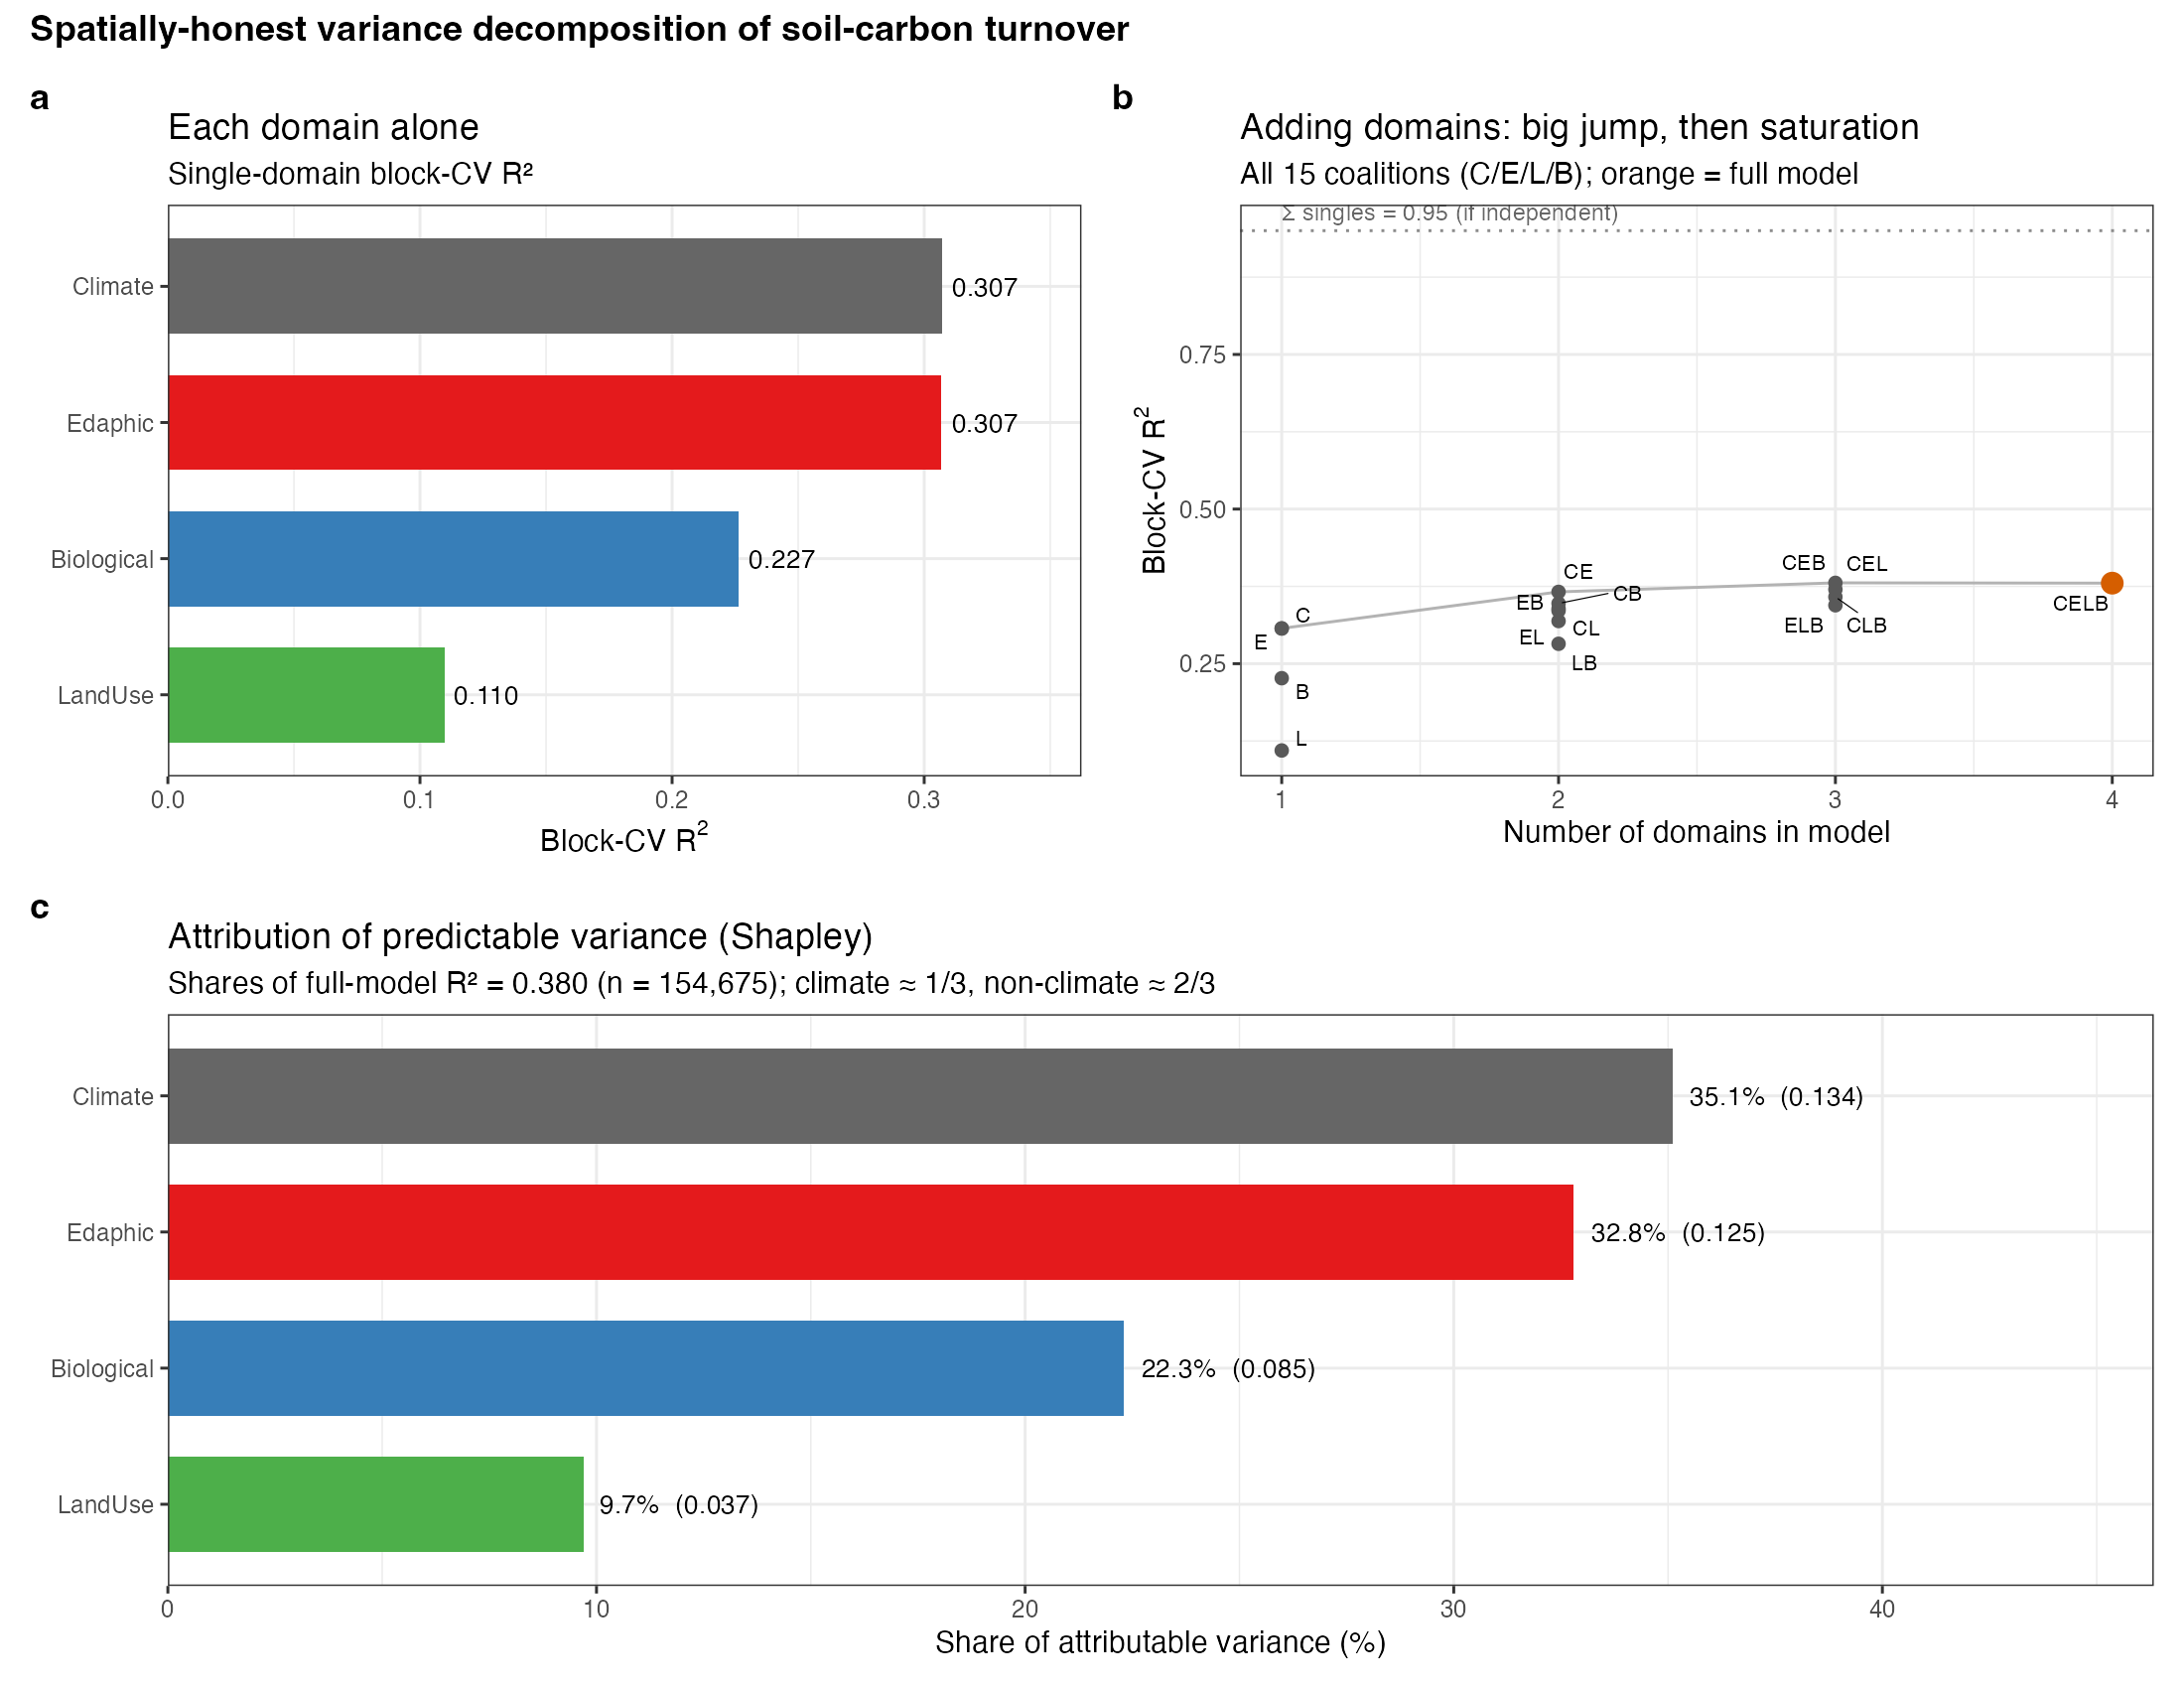
\includegraphics[width=0.92\textwidth]{../plots/step_13c_commonality/13c_decomposition.png}
\caption{\textbf{Climate explains about a third of the attributable variance in
$\tau$.} Order-independent Shapley shares (Climate~35, Edaphic~33, Biological~22,
Land use~10\,\%) with single-domain skills, on the common row set
($n=150{,}863$). The full model sits well below the sum of single-domain skills,
the overlap that marks predictors that are correlated but not redundant, an
expression of the zonal coupling between climate and soil.}
\label{fig:shapley}
\end{figure}

\begin{figure}[H]\centering
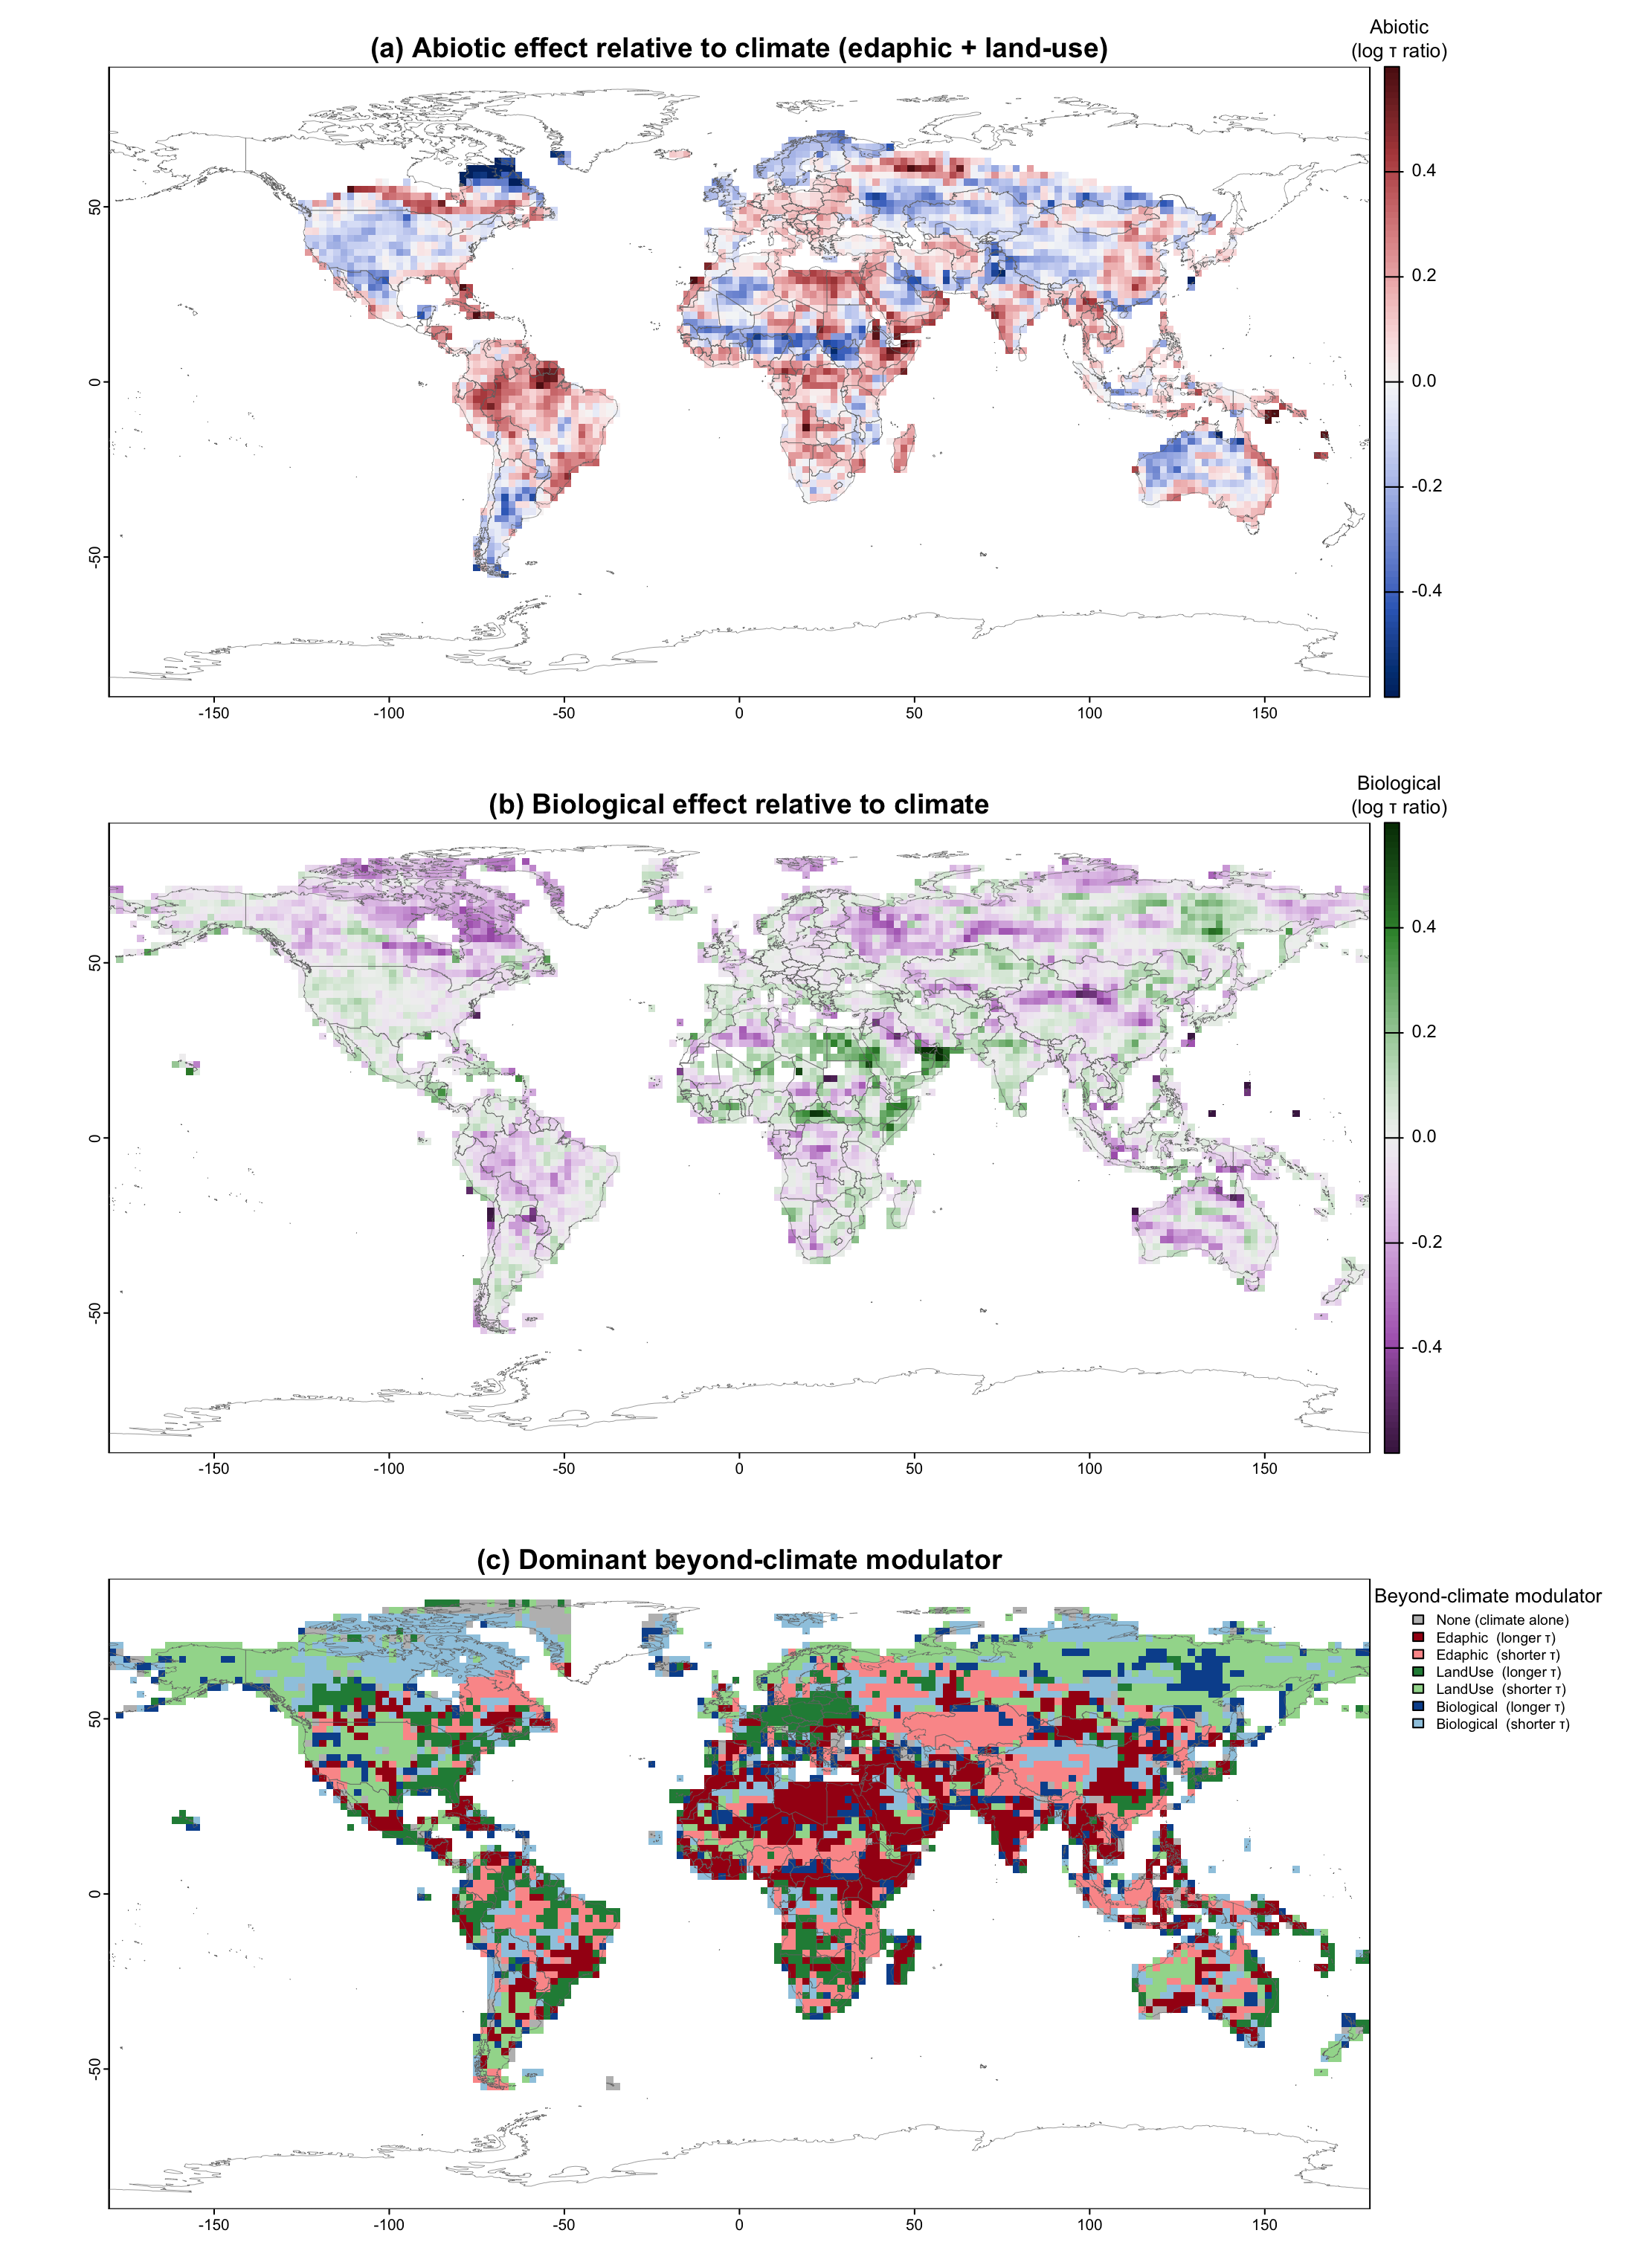
\includegraphics[width=0.95\textwidth]{../plots/step_15b_zonality/zonality_three_panel.png}
\caption{\textbf{The beyond-climate signal is zonally organised.}
(a)~Abiotic (edaphic $+$ land-use) and (b)~biological modulation of $\tau$ relative
to climate, at meso ($2^{\circ}$) scale: the log-ratio of the full-model to the
climate-only prediction per block (red/green~=~longer turnover, blue/purple~=~shorter).
The heatmap band on the left of each map is the same map collapsed onto latitude
(the zonal median across longitude, same palette and scale), the ``latitude-flat''
summary of the map beside it.
(c)~Dominant non-climate modulator per block (largest Shapley-weighted log-ratio),
shaded by direction; grey~=~climate alone. Climate is the baseline of all panels, so
a coloured block marks where a non-climate group most influences the departure from
climate, not where climate is unimportant. The organisation of the residual is
quantified by Moran's $I=0.25$ ($p\ll0.001$).}
\label{fig:zonality}
\end{figure}

\begin{figure}[H]\centering
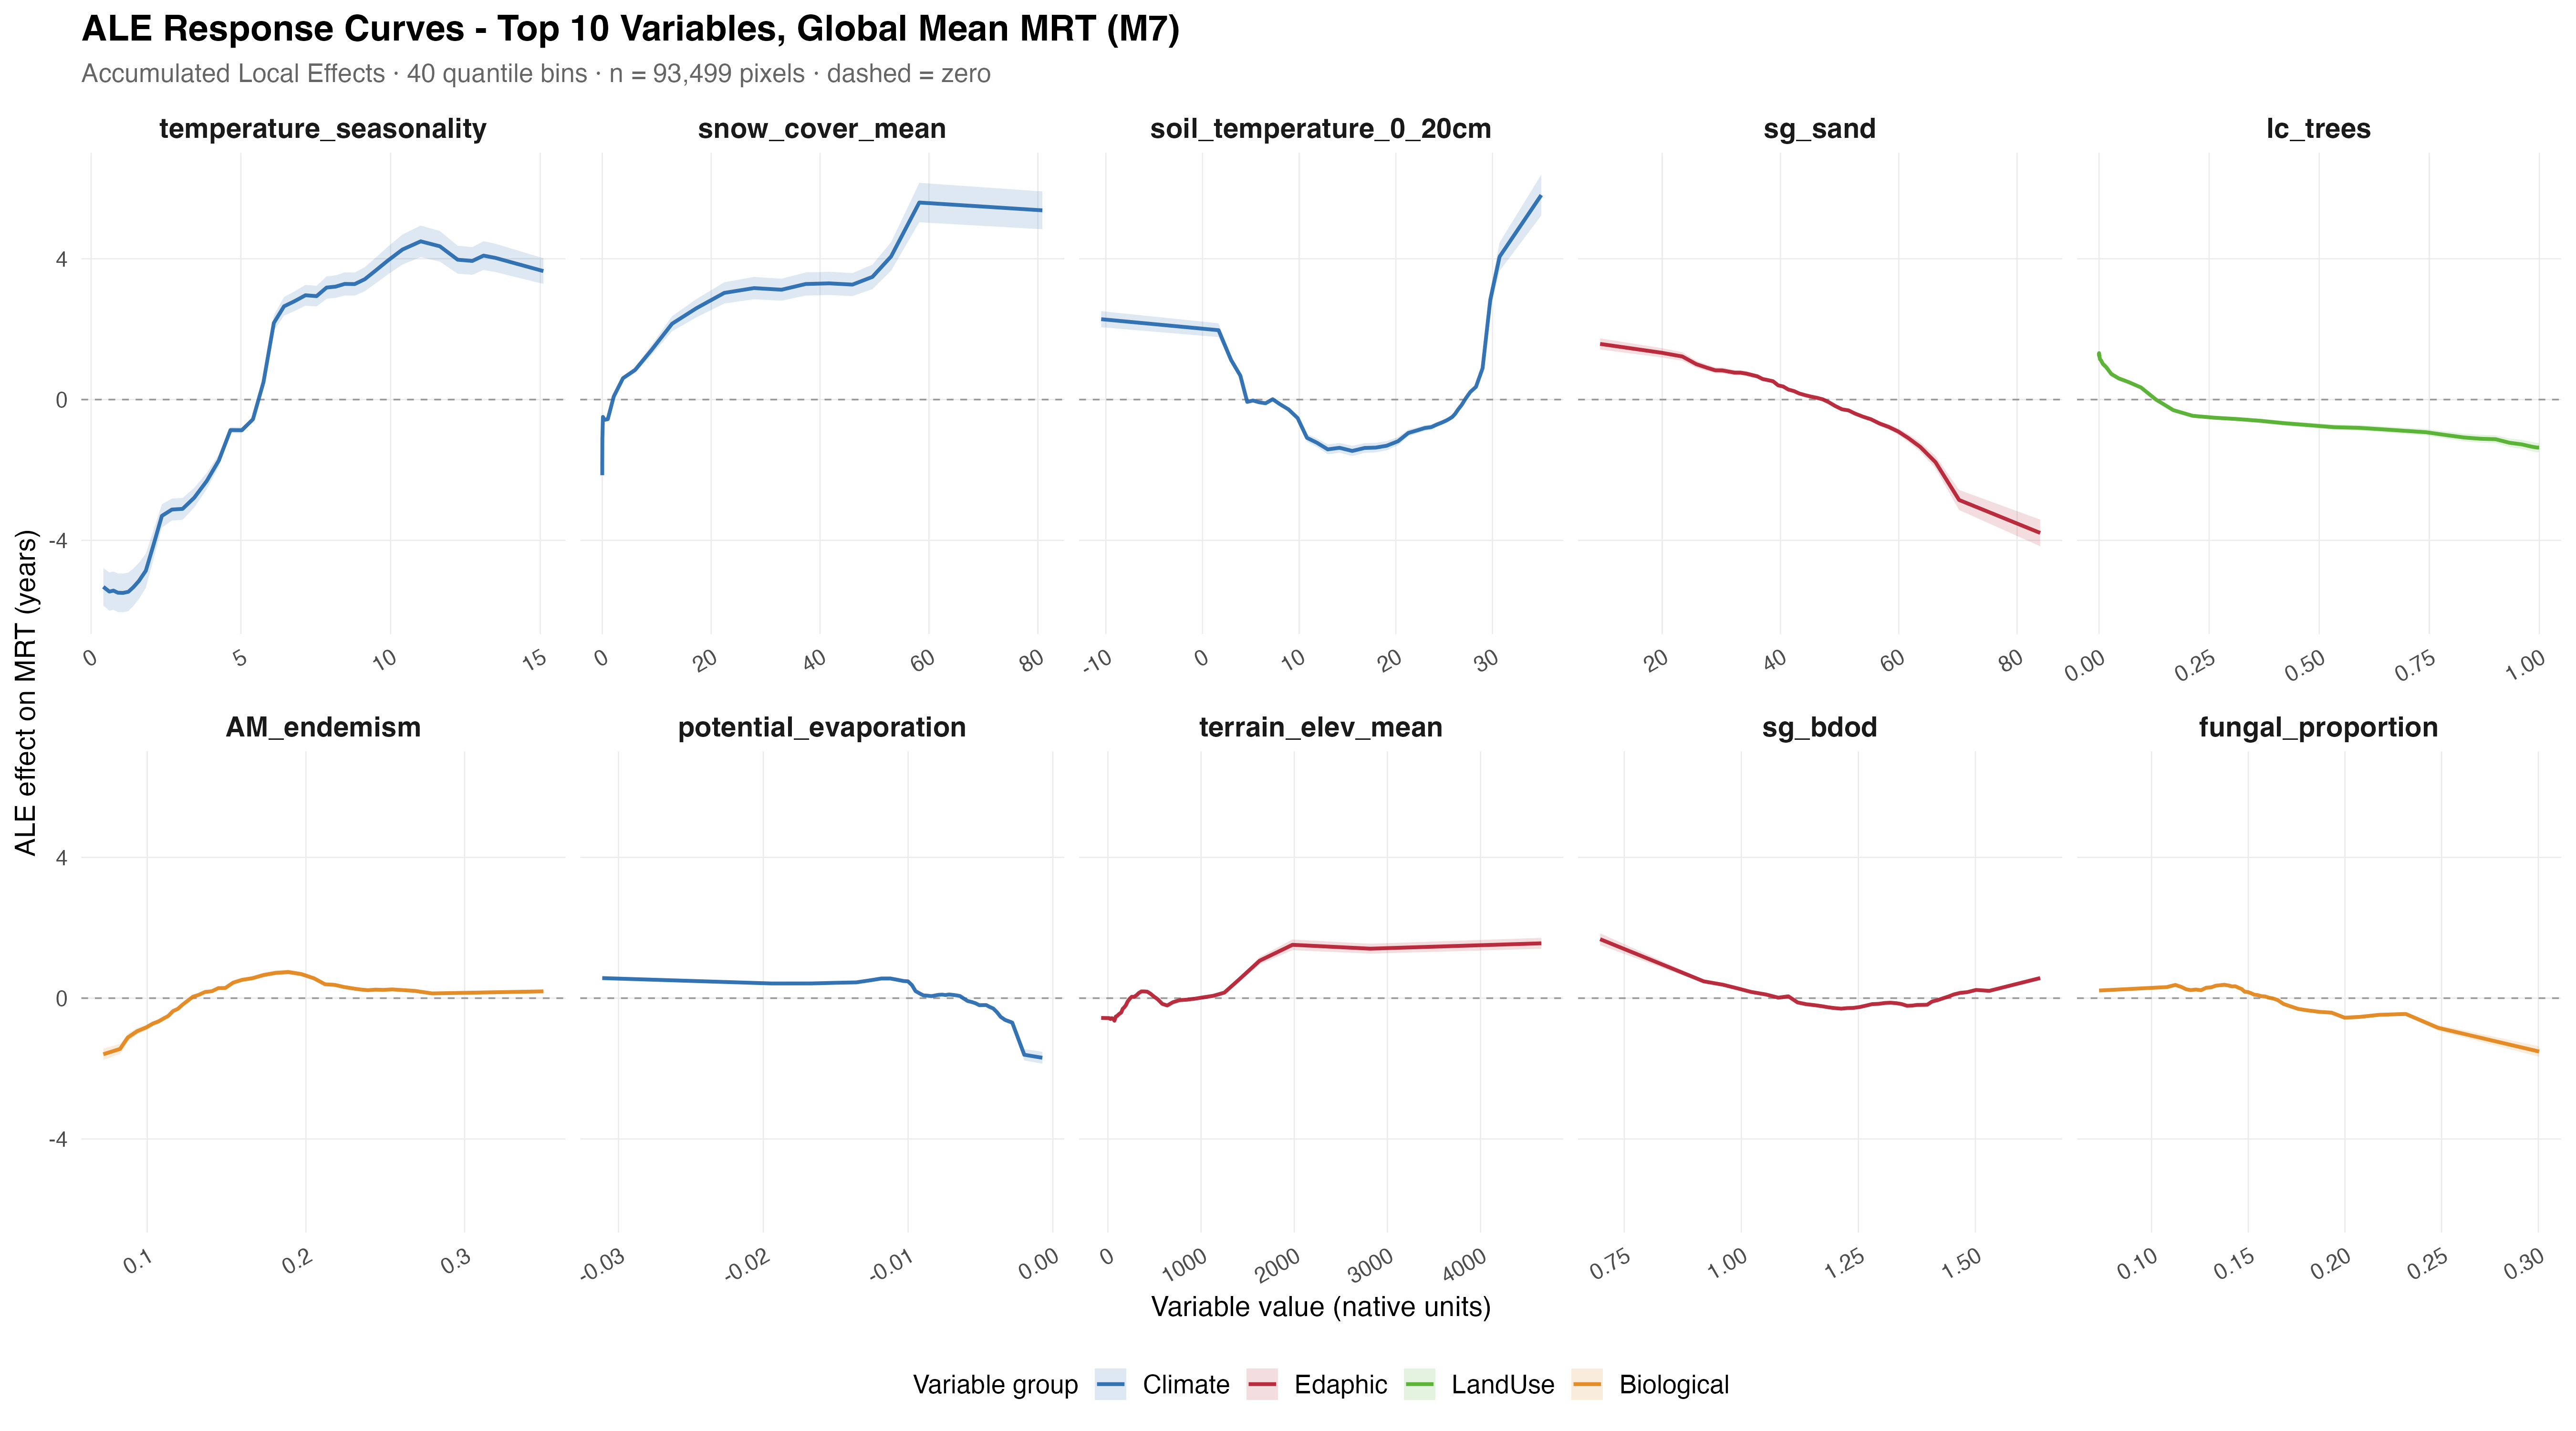
\includegraphics[width=1.0\textwidth]{../plots/step_18_sensitivity/18D_ALE_top10_MRT.png}
\caption{\textbf{Drivers act through interpretable response functions.} Accumulated Local
Effects for the ten most responsive predictors of $\tau$ (full model), ordered by
decreasing response range on a shared $y$-axis; the leaders are climatic, with sand
the strongest edaphic response. Several functions are non-monotonic and biome-dependent
(latitude-band curves in Extended Data).}
\label{fig:ale}
\end{figure}

\begin{figure}[H]\centering
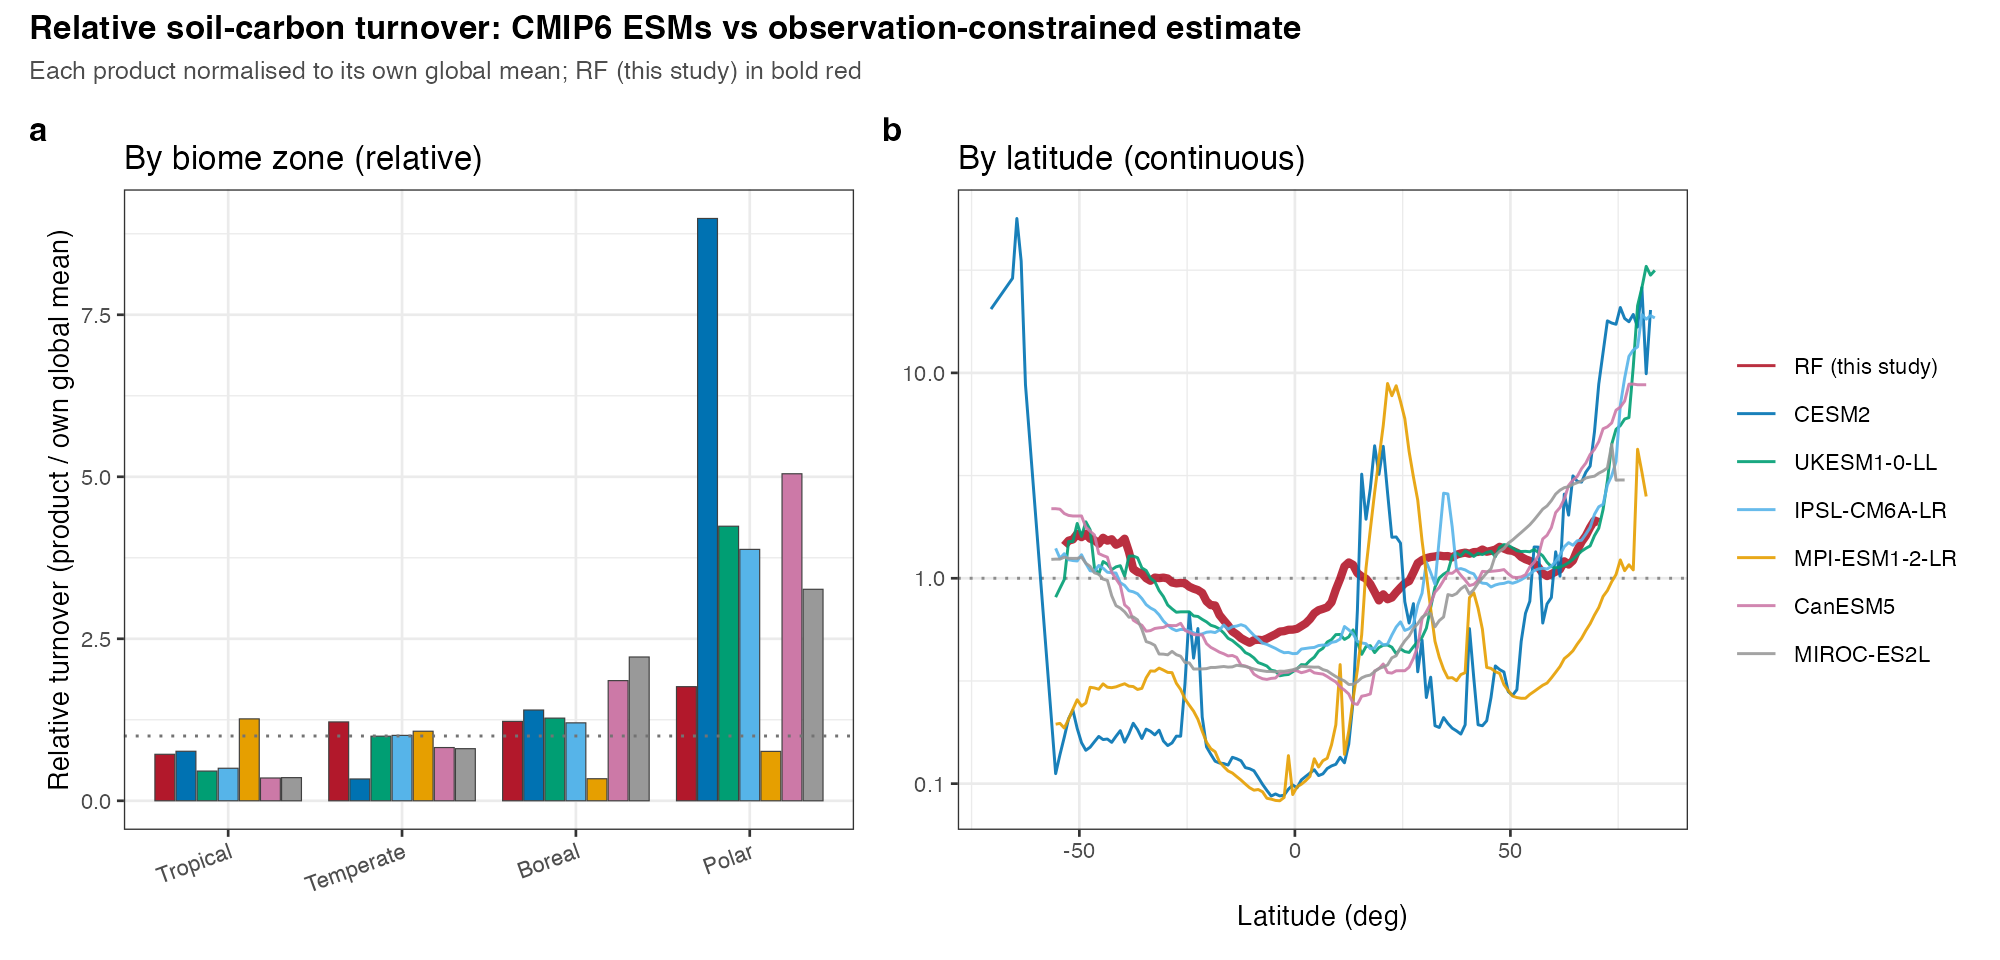
\includegraphics[width=\textwidth]{../plots/step_20/fig_esm_relative_panels.png}
\caption{\textbf{A gentler poleward gradient than Earth System Models.} Relative
soil-carbon turnover, each product normalised to its own global mean, shown (a)~by
biome zone and (b)~as continuous latitudinal profiles. Our estimate (bold red) stays
near its global mean across zones, whereas the CMIP6 models rise steeply towards the
poles (median polar/tropical contrast $\sim$9$\times$ versus $\sim$2.5$\times$ for
this study; range 0.6--14$\times$, including an inverted MPI gradient).}
\label{fig:esm}
\end{figure}

\begin{figure}[H]\centering
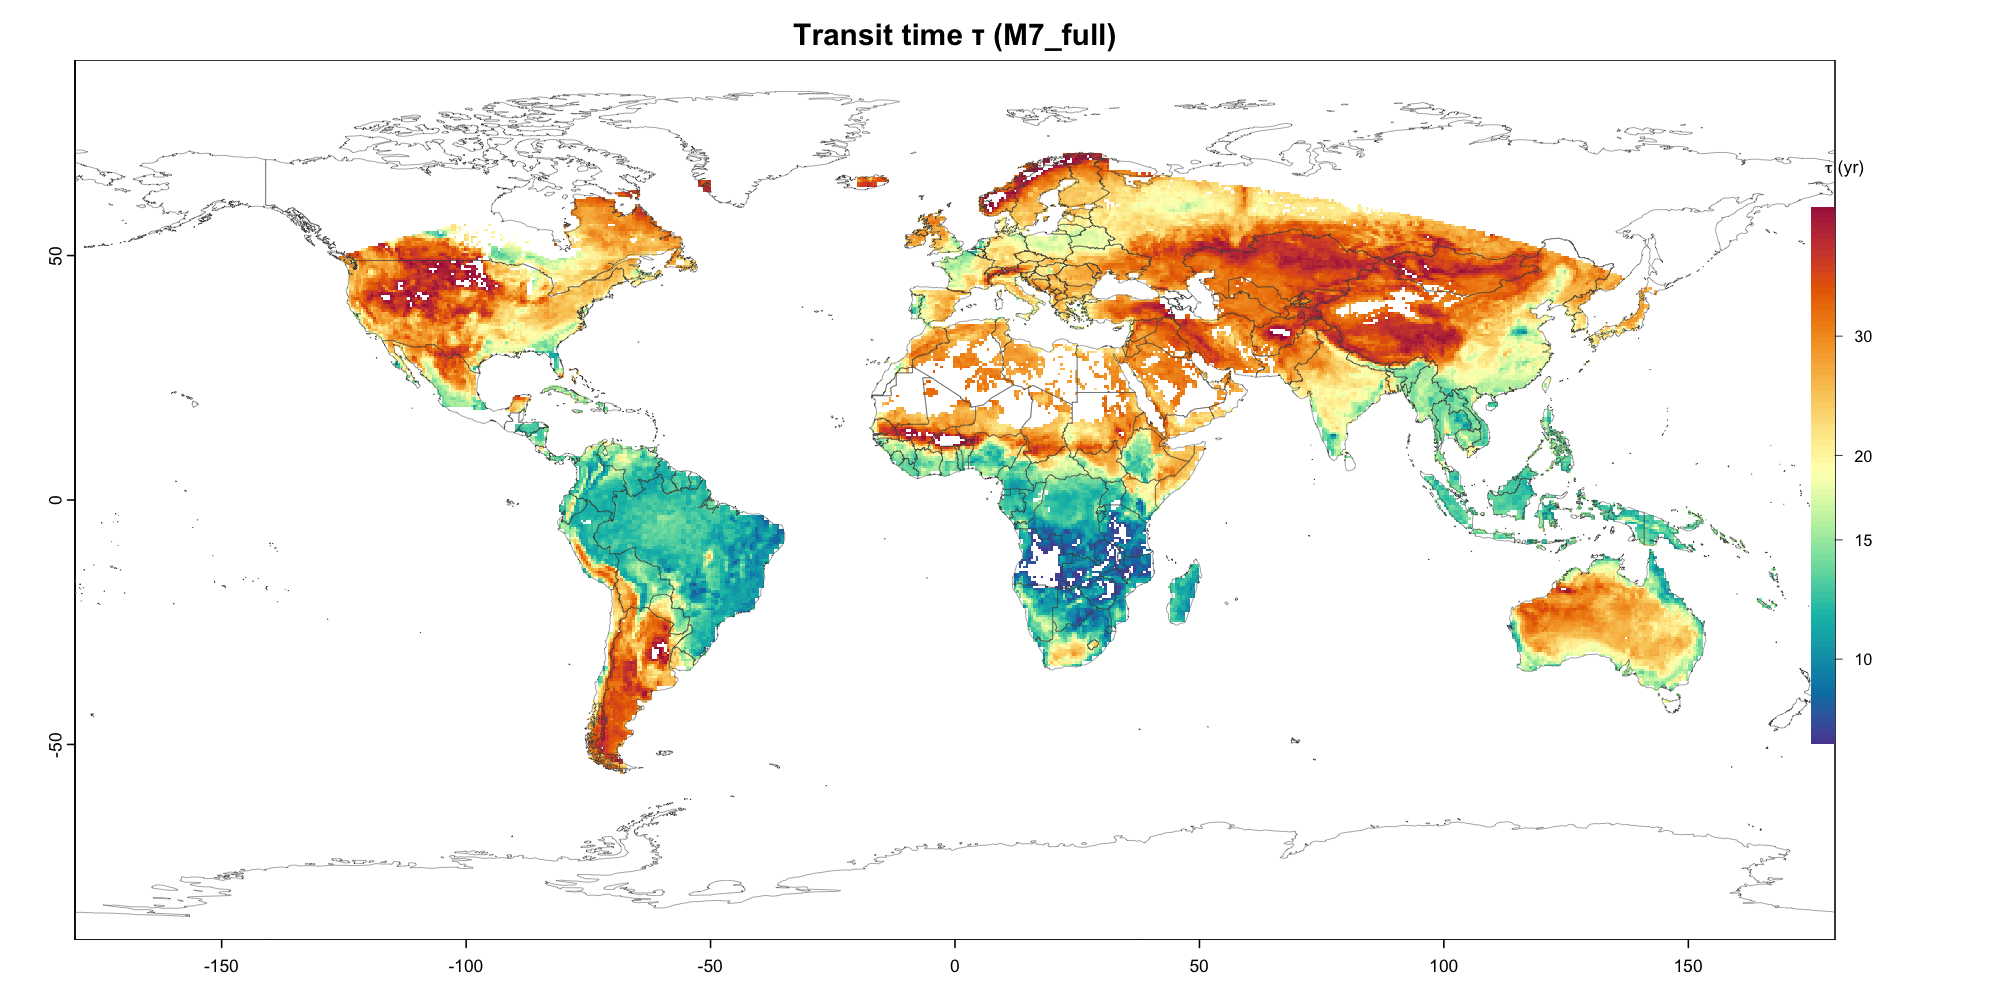
\includegraphics[width=1.0\textwidth]{../plots/step_17_visualizations/MRT_M7_full_map_log.png}
\caption{\textbf{Global distribution of predicted transit time.} Full-model
prediction at $0.1^{\circ}$ (global mean $\tau=23.5$~yr, range 3.9--72.8~yr);
log-scale palette, ticks in years. The first-order poleward gradient is consistent
with temperature control on decomposition; the beyond-climate structure of
Figs~\ref{fig:shapley}--\ref{fig:zonality} is what remains once that gradient is
removed.}
\label{fig:global_mrt}
\end{figure}

% =============================================================================
% ONLINE METHODS (Nature convention: after the main text and references; heavy
% detail devolved to Supplementary Information). Condensed from the full Methods
% of manuscript.tex; all parameters and equations preserved.
% =============================================================================
\newpage
\section*{Methods}

\noindent This section summarises the analysis; the full procedural detail (data
compilation, quality control, gap-filling, and the formal definitions of each
statistic) is given in Supplementary Methods.

\paragraph{Transit time.}
We define $\tau$ as the average time a carbon atom spends in soil from entry to exit
\citep{Sierra2017,Sierra2018}. Under steady state (constant SOC stock and input) and
a single homogeneous pool it equals the stock-to-input ratio and the inverse of the
apparent first-order rate constant,
\begin{equation}
  \tau \;=\; \frac{\text{SOC}_\text{stock}}{C_\text{input}} \;=\; \frac{1}{k}.
  \label{eq:mtt}
\end{equation}
For multi-pool systems this is a bulk diagnostic that aggregates pools of differing
rates \citep{Sierra2018}, and it is directly comparable to the transit-time
diagnostics computed from ESM output \citep{Carvalhais2014,Sierra2017}.

\paragraph{Soil data and transit-time estimation.}
Mineral-soil profiles were compiled from the OpenLandMap Open Compendium of Soil
Datasets \citep{OpenLandMapSoilDB2025}, retaining records with organic carbon
$<120$~g\,kg$^{-1}$ and depth-standardising seven properties to 0--20~cm by
thickness-weighted averaging. After quality control (removal of encoded-missing
zeros, exact duplicates, and implausible bulk density) 198{,}382 profiles remained;
bulk density was gap-filled by a Random Forest (outperforming the SoilGrids product
in ten-fold cross-validation) with a SoilGrids fallback. SOC stock was
$\text{OC}\times\text{BD}\times20\times10$ (g\,C\,m$^{-2}$). Carbon input was the
belowground fraction of MODIS MOD17A3 NPP \citep{Running2021}, using only pre-sampling
years for temporal consistency with steady state, with belowground allocation
fractions assigned by dominant land cover \citep{Mokany2006,Malhi2011,Litton2008}.
Root-derived carbon is preferentially stabilised in persistent SOC
\citep{Rasse2005,Jackson2017}, so the belowground input is a deliberate,
conservative boundary; sensitivity to this choice is examined below. After excluding
$\tau<1$ or $>1000$~yr and trimming the 1st/99th percentiles, 181{,}887 profiles
remained ($\tau$ range 1.9--143.8~yr). Observations on peat in the Global Peatland
Map 2.0 \citep{GreifswaldGPM2022} (both tiers; 6{,}922 profiles, 3.5\,\%) were
excluded from the fit, and peat and open water were masked on all maps.

\paragraph{Predictors and modelling.}
Predictors were organised into four mechanistically distinct groups (Climate,
Edaphic, Land use, Biological; Extended Data Table~\ref{edtab:predictors}), from ERA5-Land
\citep{MunozSabater2021}, K\"oppen--Geiger classes \citep{Beck2023}, SoilGrids
250\,m v2.0 \citep{Poggio2021}, the Copernicus GLO-30 DEM \citep{CopernicusDEM2022},
ESA WorldCover \citep{Zanaga2022}, Hansen forest change \citep{Hansen2013}, MODIS
burned area \citep{Giglio2018}, and mycorrhizal maps \citep{Yu2022,Barcelo2023,VanNuland2025}.
Productivity variables were excluded by design to avoid circularity with the
NPP-derived input. The biological group uses a six-layer set ($\geq96\,\%$ coverage);
three root-colonisation layers that add negligible unique skill while cutting
coverage to ${\sim}62\,\%$ enter only a sensitivity check. All models were fitted with \texttt{ranger}
\citep{Wright2017} on $\ln\tau$.

\paragraph{Spatially-honest skill and attribution.}
Predictive skill is reported as spatial-block cross-validated $R^2$: the globe was
partitioned into $2^{\circ}$ ($\sim$200~km) blocks assigned to ten folds, each
fold predicted from a model trained on the others, so that a held-out region is not
propped up by an almost-coincident training neighbour (the residual stays correlated
only to $\approx24$~km). Enlarging the block to $1^{\circ}$ or $5^{\circ}$ lowers absolute
skill but shifts each group's attributed share by at most 2 percentage points. To
attribute the explained variance among the four correlated groups we use a Shapley
decomposition: fitting all $2^4=16$ group subsets on a common row set and averaging
each group's marginal contribution over all orders of entry,
\begin{equation}
  \phi_i = \!\!\sum_{S\subseteq N\setminus\{i\}}
  \frac{|S|!\,(|N|-|S|-1)!}{|N|!}\,[\,v(S\cup\{i\})-v(S)\,],
  \label{eq:shapley}
\end{equation}
where $v(S)$ is the cross-validated $R^2$ of the model on subset $S$; the $\phi_i$
sum to the full-model $R^2$ and are reported as percentage shares. The same
decomposition was repeated within contiguous $10^{\circ}$ latitude bands,
refitting every subset with local block cross-validation inside each band (bands with
fewer than 800 observations or 40 blocks were left unattributed), to test whether the
attribution itself is zonally structured; because each band removes the between-band
gradient, these shares reflect within-band spatial structure rather than the
latitudinal level (Extended Data Fig.~\ref{edfig:latshapley}).

\paragraph{Organisation, mapping and mechanism.}
Spatial organisation of the beyond-climate residual (out-of-sample $\ln\tau$ minus
the climate-only prediction, aggregated to blocks) was tested with Moran's $I$ using
row-standardised $k=8$ nearest-neighbour weights against 999 permutations, at
$2^{\circ}$ and $5^{\circ}$. The zonality map is the log-ratio
$\ln[\hat\tau_\text{context}/\hat\tau_\text{climate}]$, computed symmetrically for
the abiotic and biological domains; the discrete zonation labels each block by its
largest Shapley-weighted modulation, or "climate alone" below a small threshold. The
mapping scale ($2^{\circ}$) was set by an out-of-sample skill curve (agreement of
mapped with observed residual rising from $\approx0.10$ native to $\approx0.23$ and
plateauing across 1--7\textdegree) and by the residual variogram (nugget/sill
$\approx0.53$, range $\approx24$~km). Marginal responses use ALE \citep{Apley2020}
on the full model (40 quantile bins), computed globally and within four latitude
bands.

\paragraph{ESM comparison and robustness.}
We compared the normalised spatial structure of our $\tau$ against six CMIP6 models
\citep{Varney2022} with $\tau_\text{ESM}=\text{cSoil}/\text{rh}$
\citep{Koven2017,Carvalhais2014} over 1980--2014, treating no product as truth and
reporting magnitude-free dispersion and a polar-to-tropical ratio. Robustness checks
(Supplementary Information) bound the main claims: a provenance control (only 2.5\,\%
of residual variance between source databases), biological parsimony, block-size
invariance, and a carbon-input convention sweep. Because the input is set by a
coefficient on one NPP field, a spatially uniform change only rescales $\tau$ and
leaves every scale-invariant quantity (block-CV $R^2$, Shapley shares, Moran's $I$)
unchanged; re-deriving $\tau$ under total-NPP and generous forest-harvest conventions
moves only the land-use share, and the beyond-climate gap is if anything slightly
larger under harvest (Extended Data Fig.~\ref{edfig:input}, Table~\ref{edtab:input}).

\paragraph{Software and data.}
Analyses used R ($\geq4.3$) with \texttt{terra}, \texttt{sf}, \texttt{ranger}
\citep{Wright2017} and \texttt{gstat}; the pipeline is a sequence of numbered
scripts and each reported number regenerates from a named script. Code and
intermediate outputs are archived at \PH{[DOI]}. Data sources are listed in the Data
availability statement.

% =============================================================================
\section*{Data availability}
Soil profiles: OpenLandMap Open Compendium \citep{OpenLandMapSoilDB2025},
\url{https://zenodo.org/records/15593990}. ERA5-Land: Copernicus CDS. SoilGrids:
ISRIC. ESA WorldCover, Hansen forest change and MODIS products from their respective
repositories; microbial datasets as cited.

\section*{Code availability}
The complete R pipeline is archived at \PH{[DOI/repository]}.

\section*{Acknowledgements}
Carried out within the NextGenCarbon project (Horizon Europe grant No.~101184989).
\PH{[further acknowledgements TBD]}

\section*{Author contributions}
\textbf{L.M.} conceived and designed the study, carried out the analysis, and wrote
the manuscript. \textbf{S.H.}, \textbf{A.L.} and \textbf{E.B.} contributed to design
choices during the work and to revision of the manuscript.

\section*{Competing interests}
The authors declare no competing interests.

% =============================================================================
\bibliographystyle{apalike}
\bibliography{references}
% =============================================================================

% =============================================================================
% EXTENDED DATA (integral to the article; Nature allows up to 10 items, figures
% and tables combined, each cited in the main text). Numbered "Extended Data
% Fig./Table". Overflow items live in the Supplementary Information
% (main_Nature_SI.tex).
% =============================================================================
\newpage
\renewcommand{\figurename}{Extended Data Fig.}
\renewcommand{\tablename}{Extended Data Table}
\setcounter{figure}{0}
\setcounter{table}{0}

\section*{Extended Data}

\begin{figure}[H]\centering
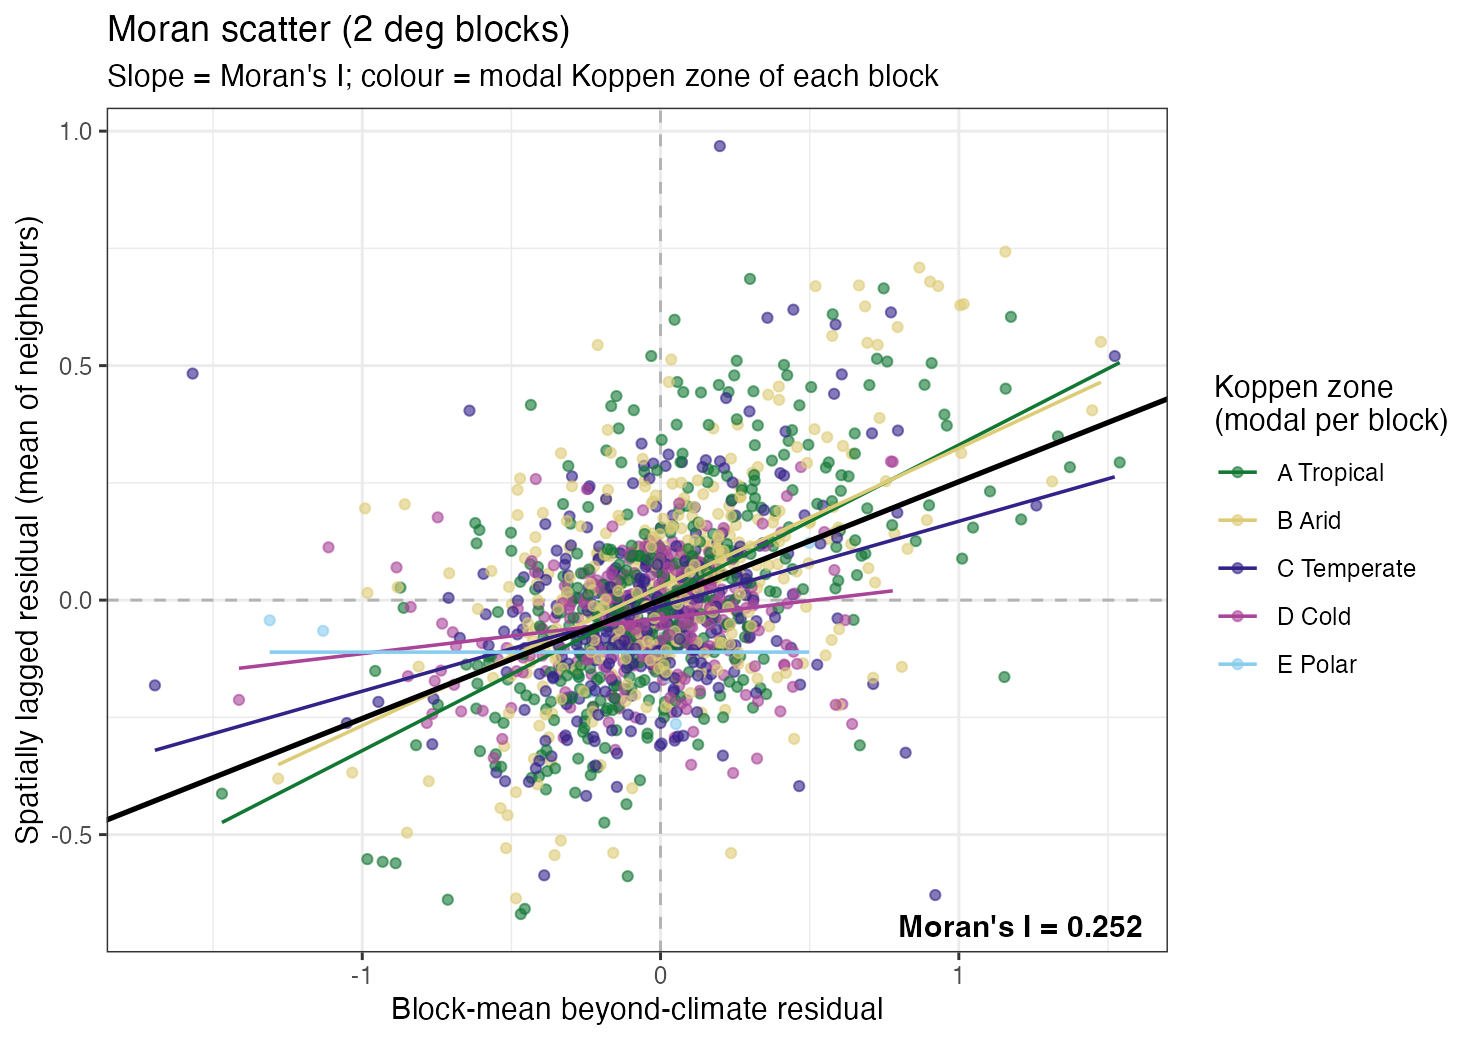
\includegraphics[width=0.6\textwidth]{../plots/step_13c_commonality/13e_moran_scatter.png}
\caption{\textbf{Spatial organisation of the beyond-climate residual.} Each point is
a $2^{\circ}$ block; horizontal axis is the block's mean beyond-climate residual
(observed minus climate-only prediction), vertical axis the average residual of its
neighbouring blocks. The positive slope is Moran's $I=0.25$ ($p\ll0.001$); a flat
cloud would indicate no organisation. Points coloured by modal coarse K\"oppen zone,
with within-zone fits: the autocorrelation is present across zones (steepest in
tropical and arid blocks, flat in the few polar blocks).}
\label{edfig:moran}
\end{figure}

\begin{figure}[H]\centering
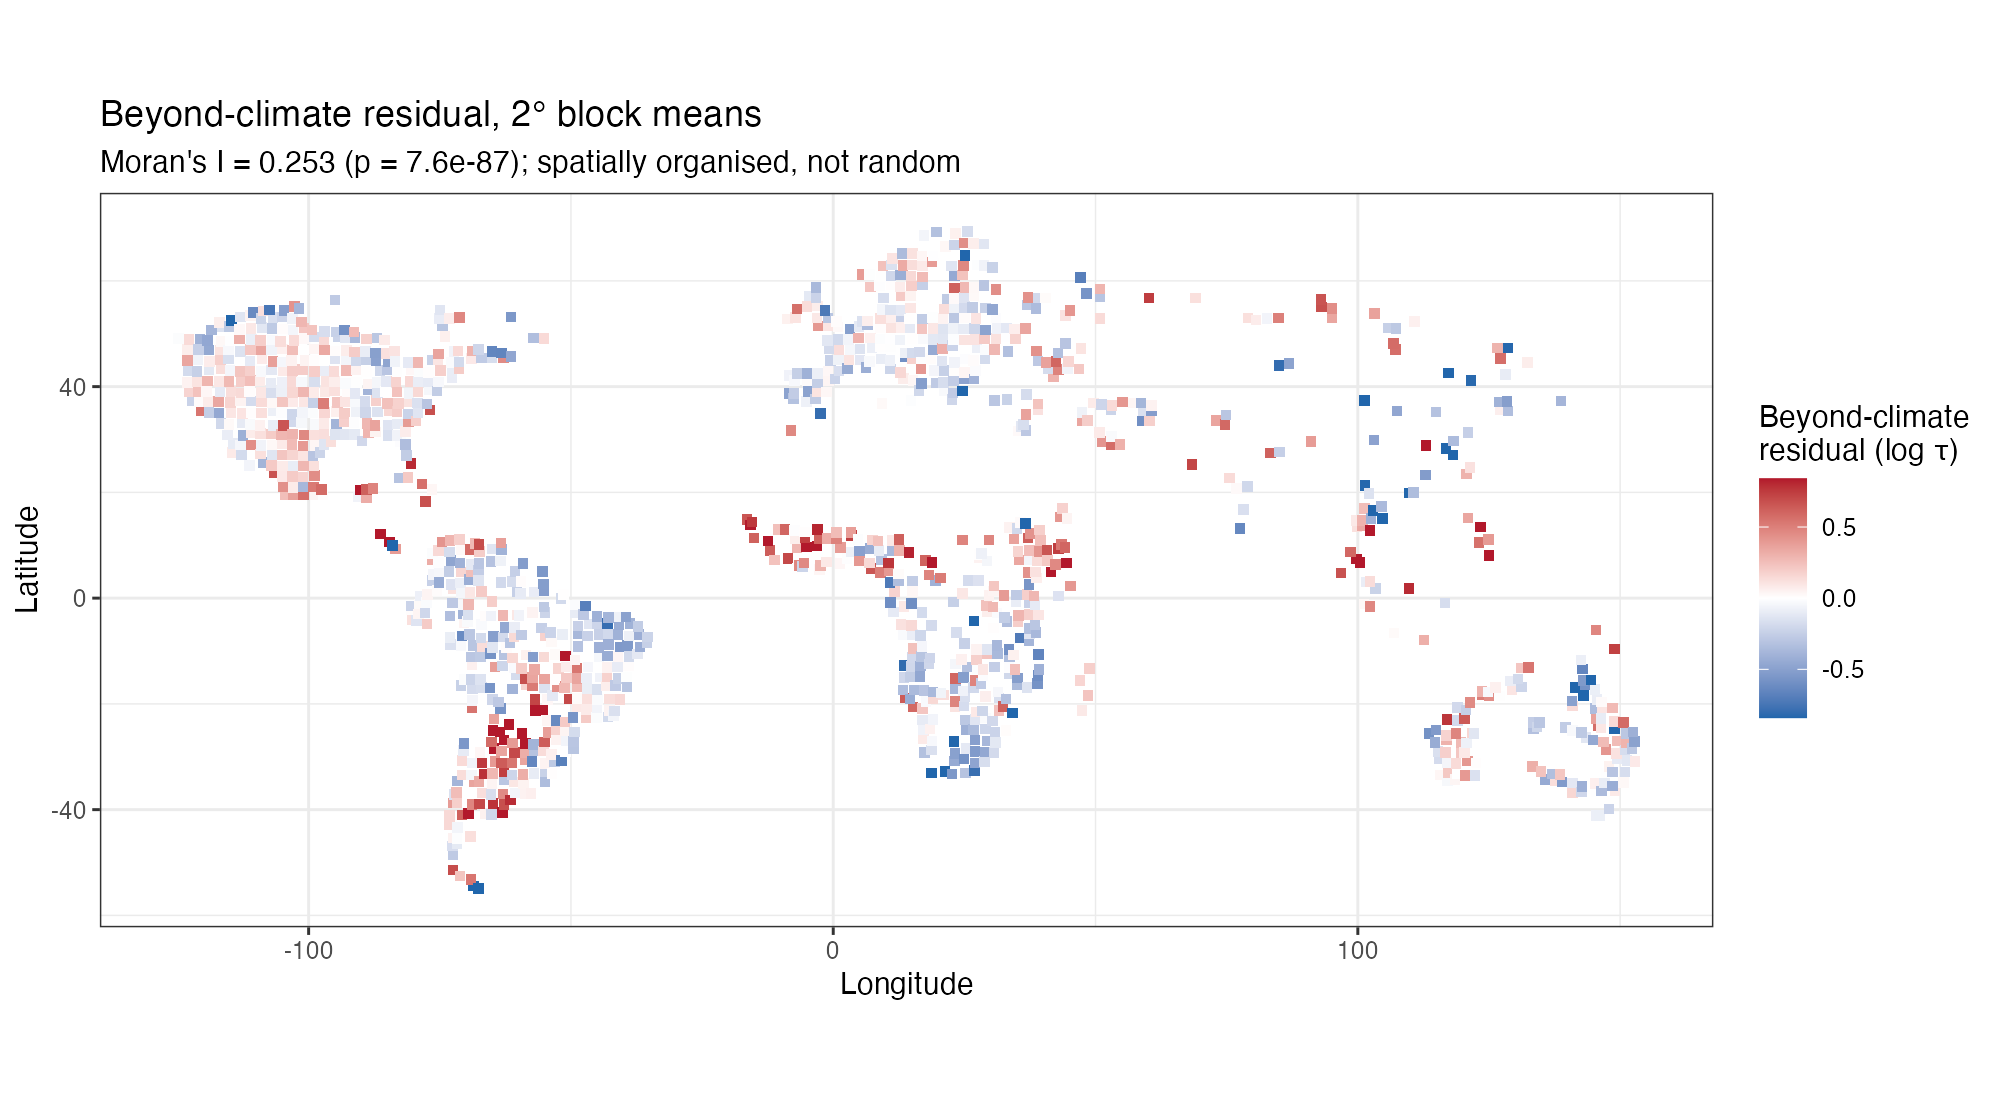
\includegraphics[width=0.85\textwidth]{../plots/step_13c_commonality/13e_block_residual_map.png}
\caption{\textbf{Beyond-climate residual map.} Block-mean beyond-climate residual
(the geographic companion to the Moran scatter, Extended Data
Fig.~\ref{edfig:moran}).}
\label{edfig:residmap}
\end{figure}

\begin{figure}[H]\centering
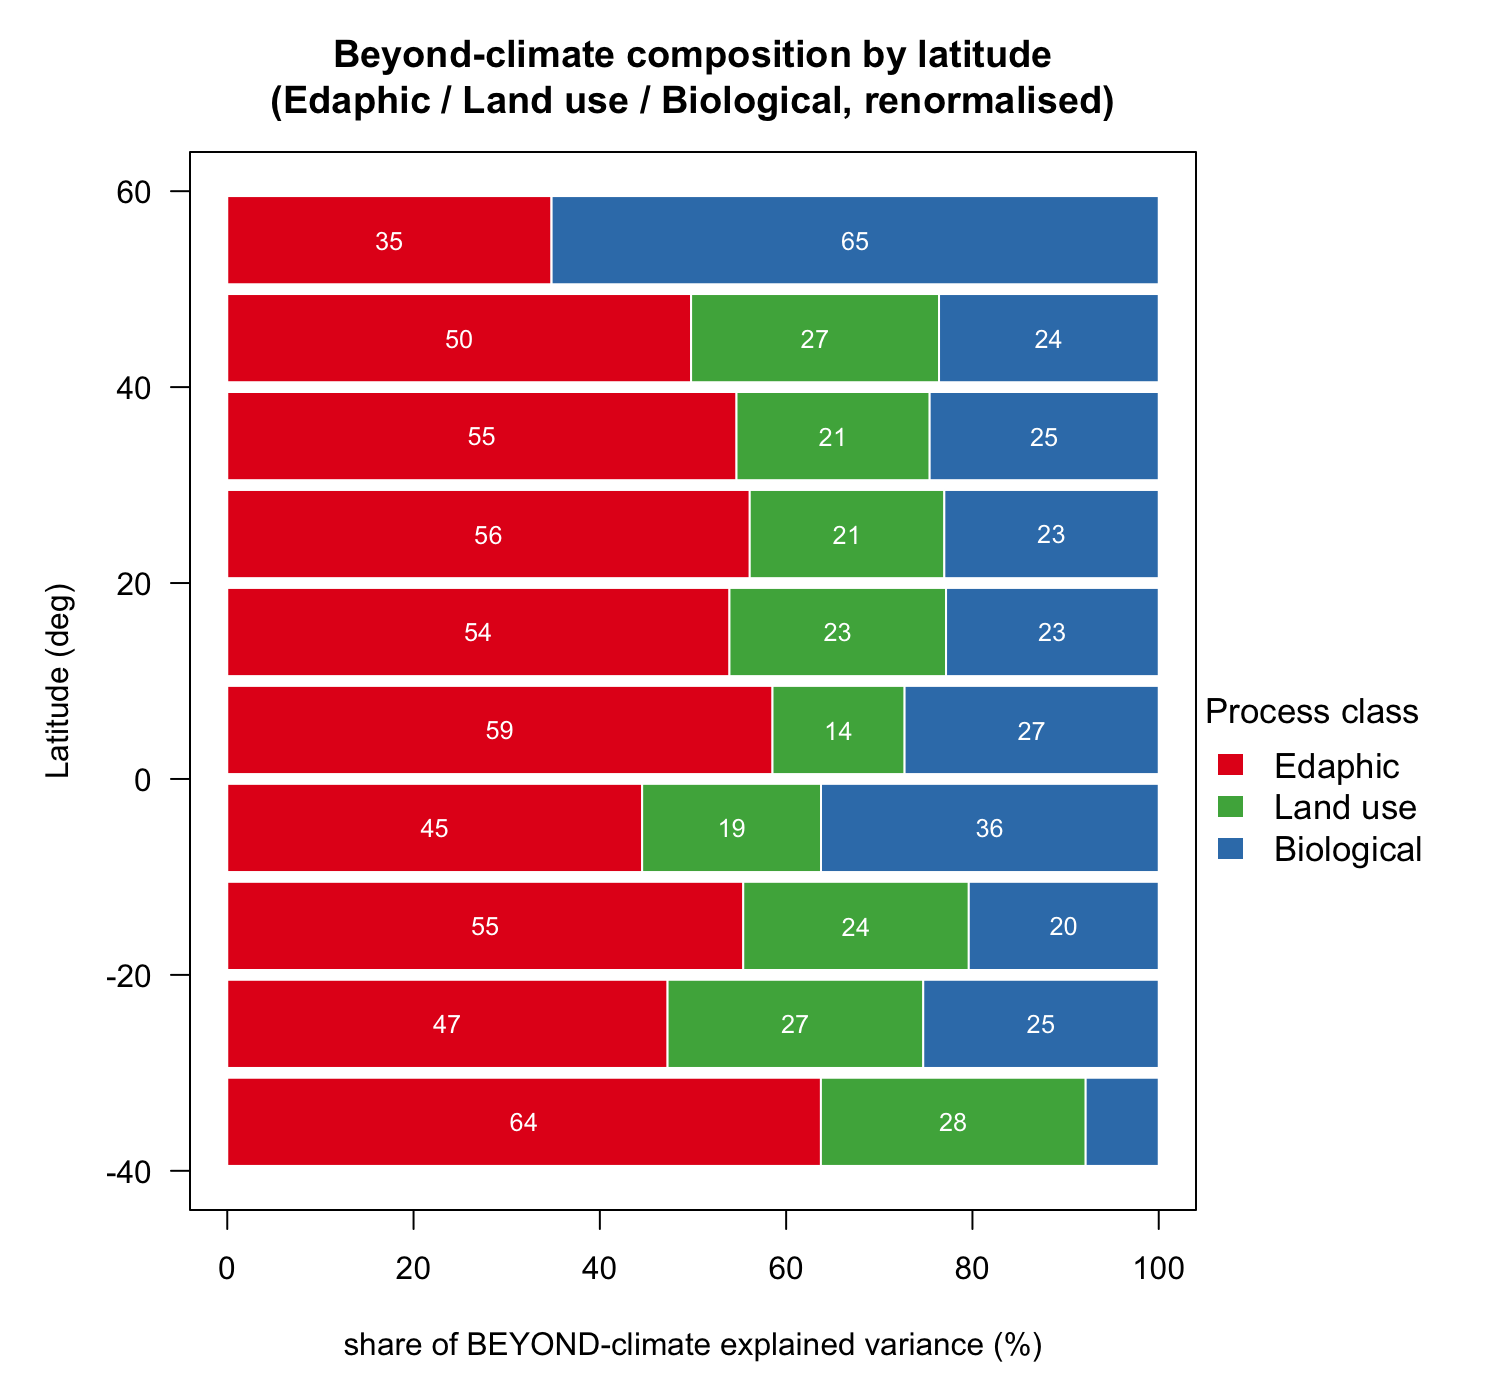
\includegraphics[width=0.72\textwidth]{../plots/step_13c_commonality/13l_beyondclimate_composition.png}
\caption{\textbf{The beyond-climate attribution is zonally structured.} The Shapley
decomposition (Methods) refit within contiguous $10^{\circ}$ latitude bands, shown
as the composition of the beyond-climate explained variance among the three
non-climate classes (Edaphic, Land use, Biological), renormalised to 100\% per band.
Edaphic context leads at nearly every latitude; soil biology rises in the humid
equatorial belt and dominates the boreal; land use is modest and never leading, and
vanishes in the boreal (its local Shapley value there is slightly negative and set to
zero before renormalising). Bands below the reliability thresholds (far southern,
$>60^{\circ}$N) are omitted. Because each band's decomposition removes the poleward
gradient, these shares describe within-band spatial structure, not the cross-latitude
level.}
\label{edfig:latshapley}
\end{figure}

\begin{figure}[H]\centering
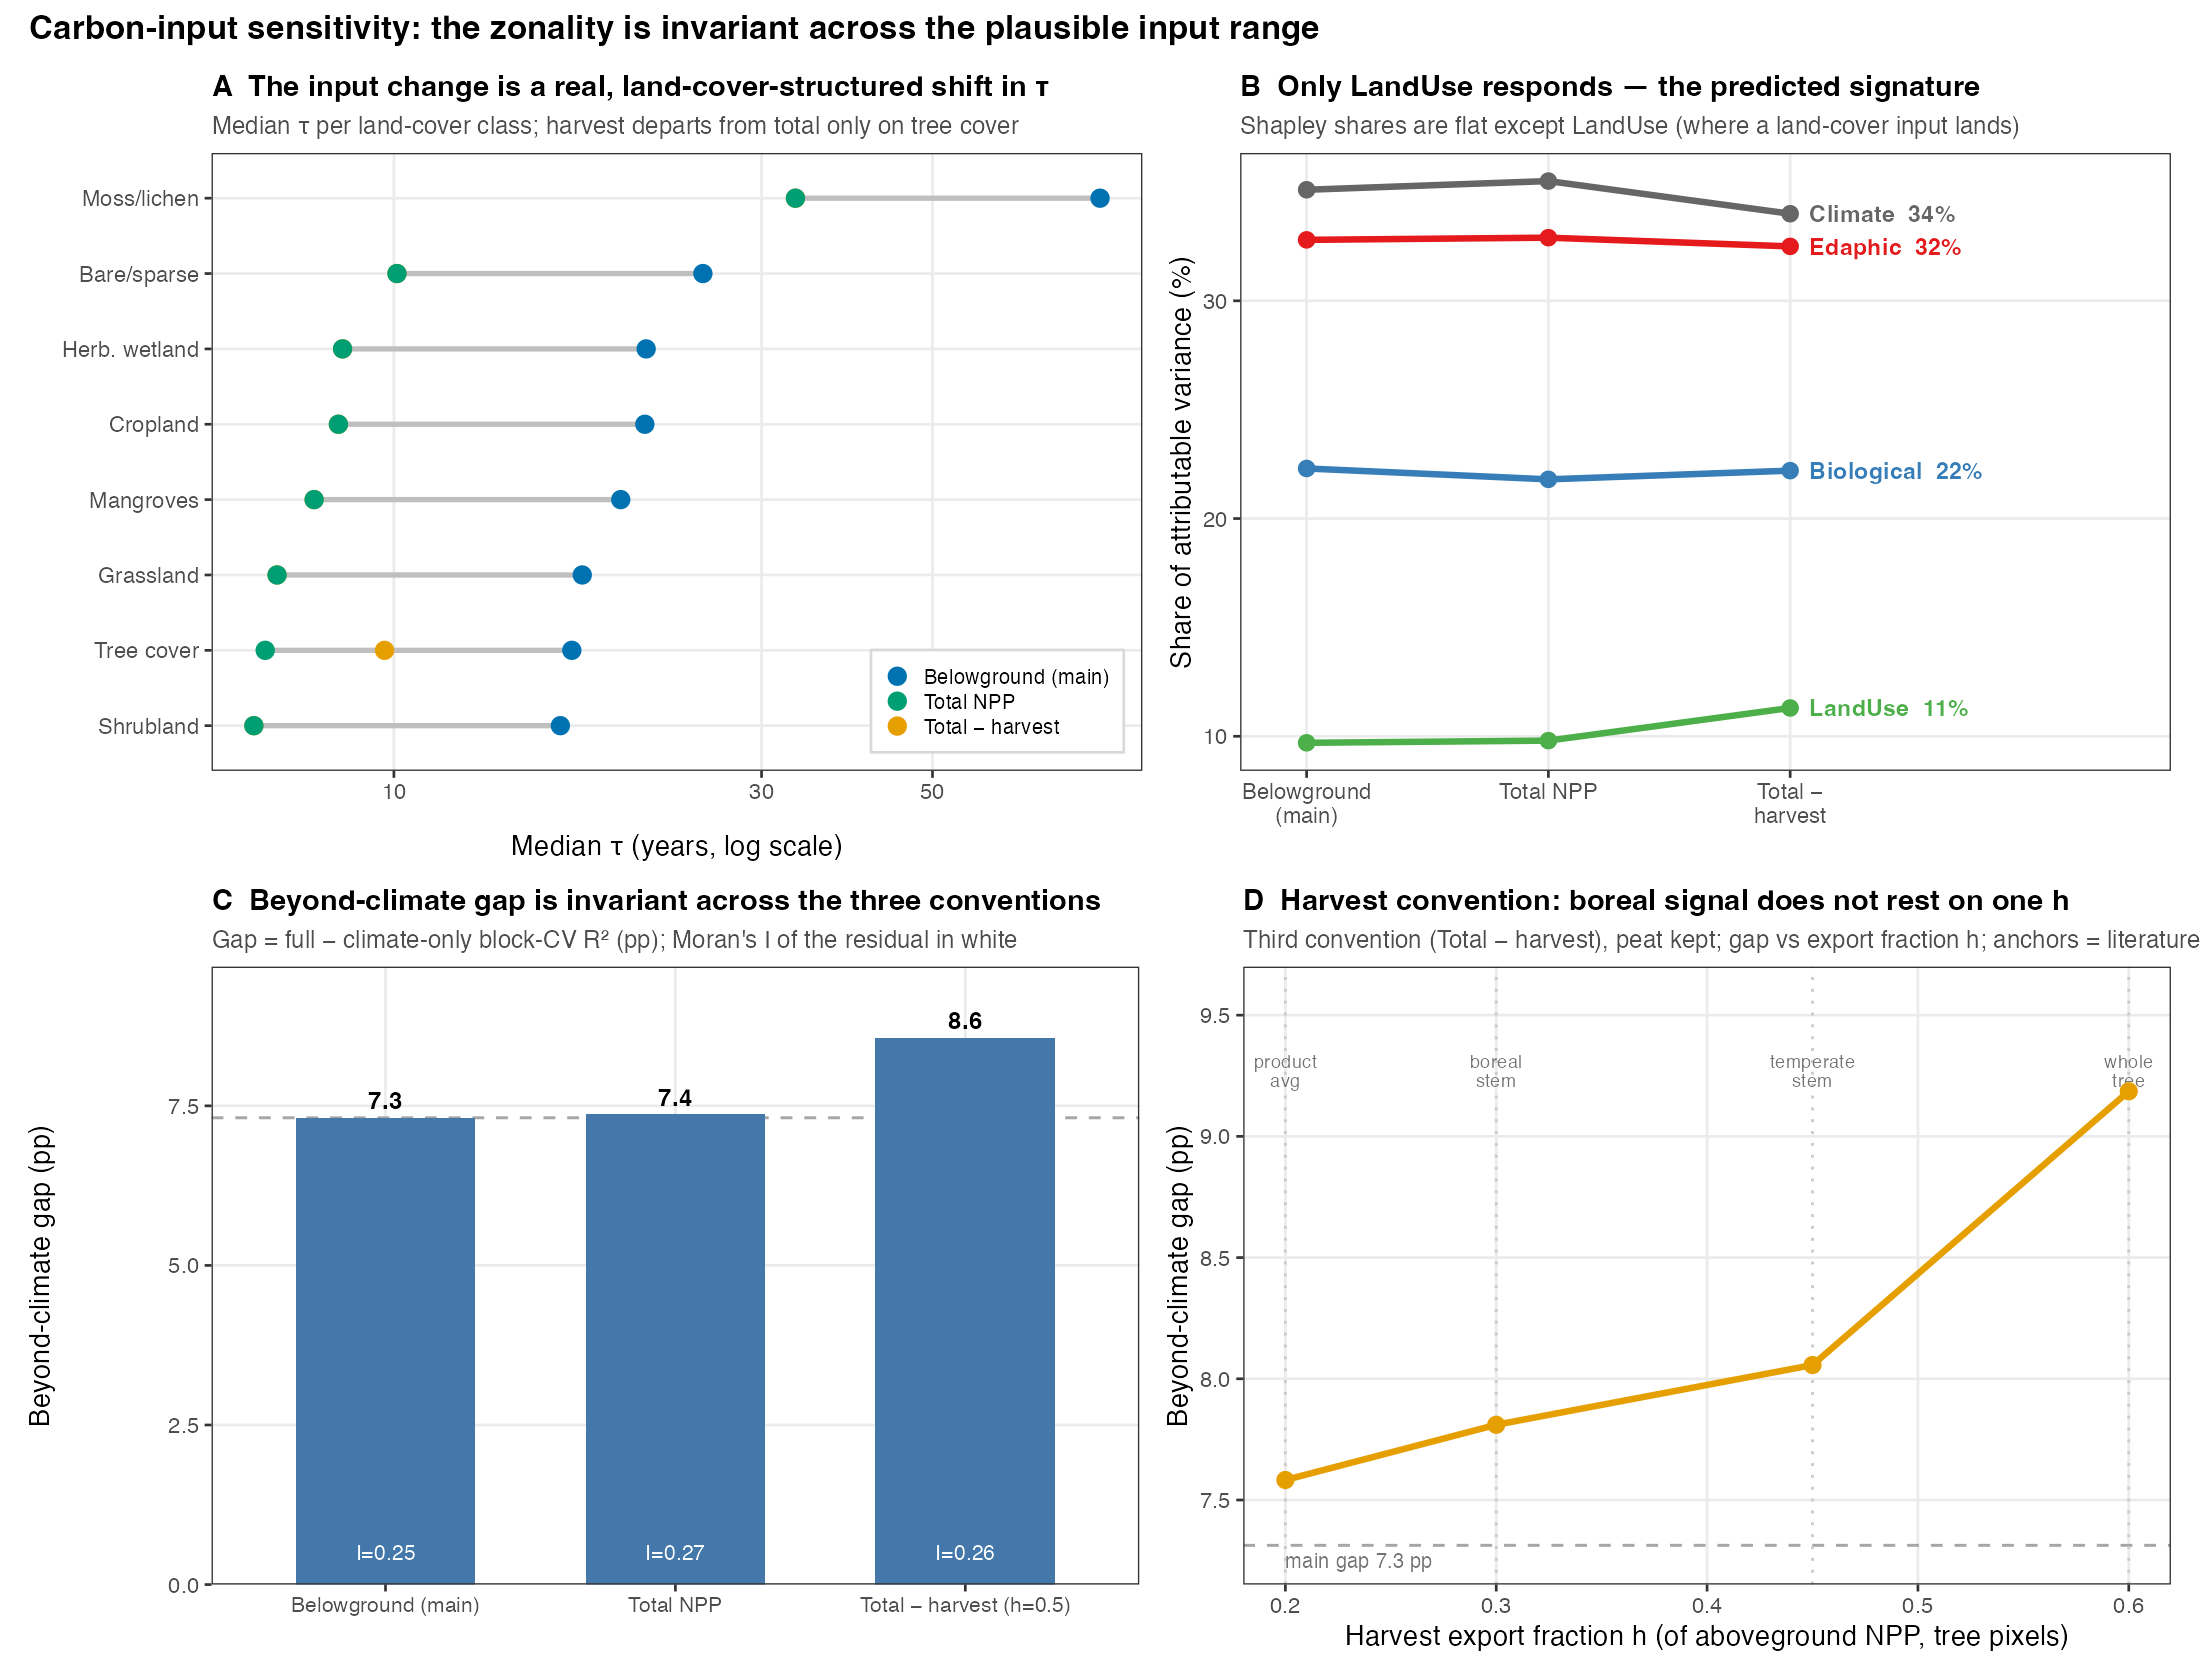
\includegraphics[width=\textwidth]{../plots/step_13c_commonality/13k_input_sensitivity_appendix.png}
\caption{\textbf{Carbon-input convention sensitivity.} The soil-carbon-input
coefficient is re-derived on the same NPP field under three conventions.
\textbf{(A)}~Median $\tau$ per land-cover class (harvest departs from total only on
tree cover). \textbf{(B)}~Shapley shares are flat across conventions except land use.
\textbf{(C)}~The beyond-climate gap and the residual Moran's $I$ (inset) are
invariant. \textbf{(D)}~For the harvest convention, the gap does not fall as the
export fraction $h$ is swept across its literature range.}
\label{edfig:input}
\end{figure}

\begin{figure}[H]\centering
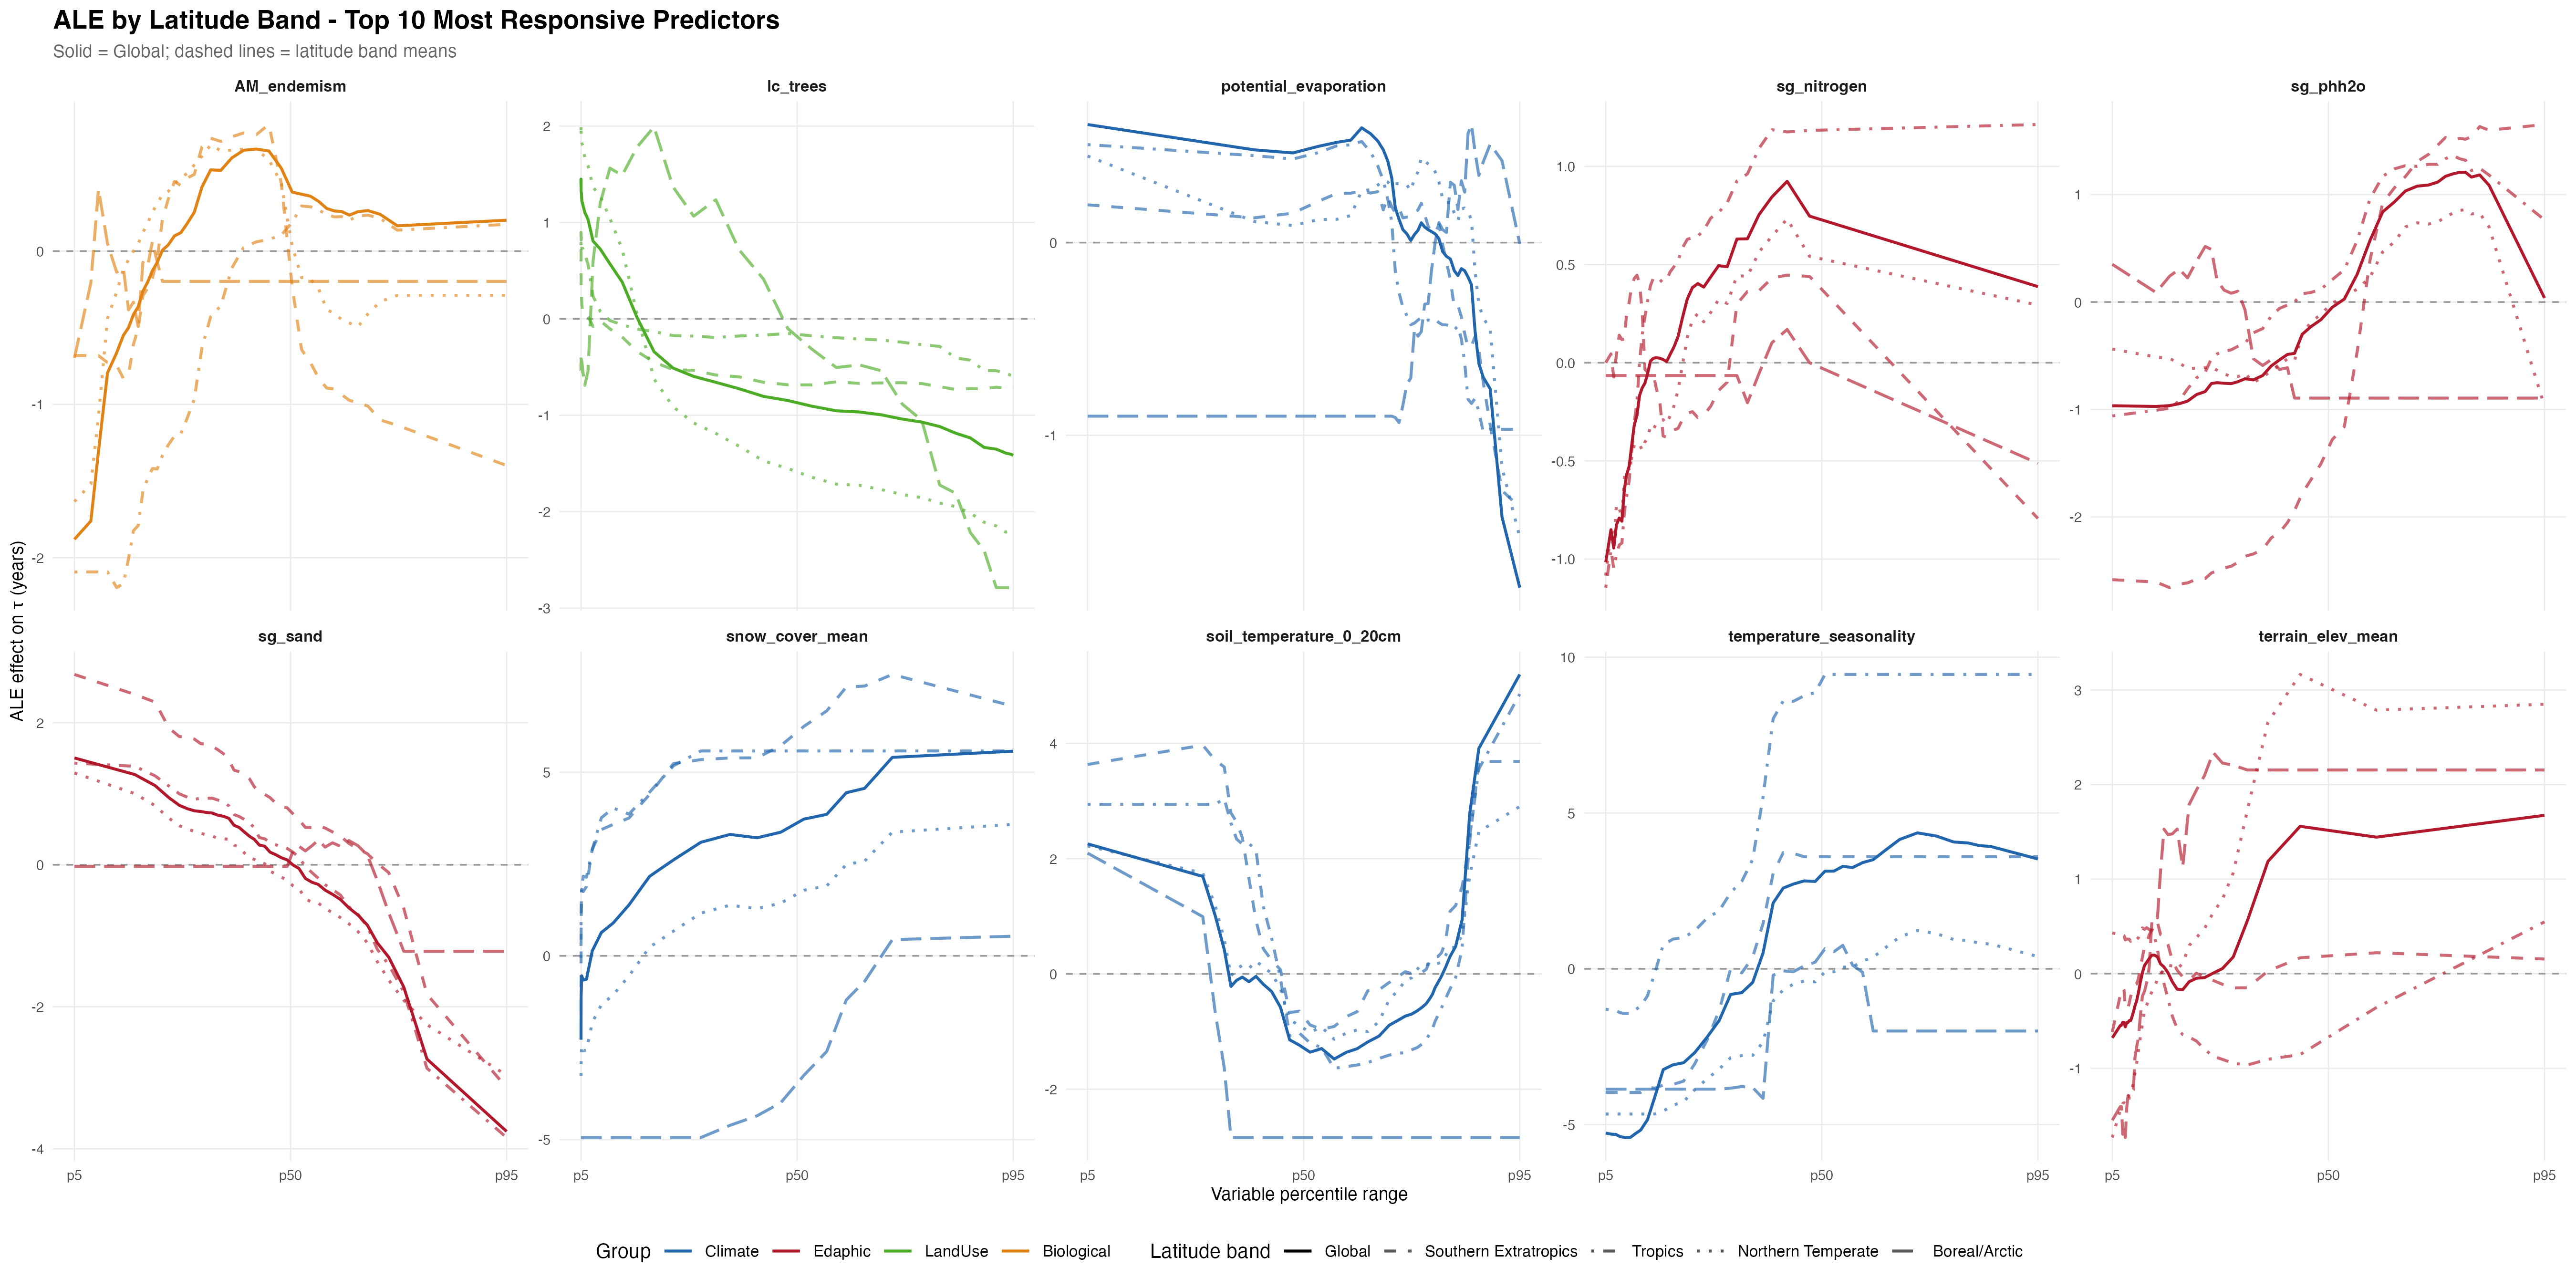
\includegraphics[width=0.95\textwidth]{../plots/step_18_sensitivity/18C_ALE_by_latband.png}
\caption{\textbf{Marginal responses by latitude band.} ALE curves for $\tau$,
computed globally and within four latitude bands (southern temperate, tropics,
northern temperate, boreal/Arctic). These underlie the biome-dependence noted in the
main text: the temperature-seasonality response is largest in the tropics, the pH
response steepest in the boreal/Arctic, and the biological responses smallest in
magnitude throughout. Bands cover different parts of each driver's range (curves are
drawn only where a band has data), so the climatic curves in particular should be
compared over the interval the bands share.}
\label{edfig:ale_latband}
\end{figure}

\begin{figure}[H]\centering
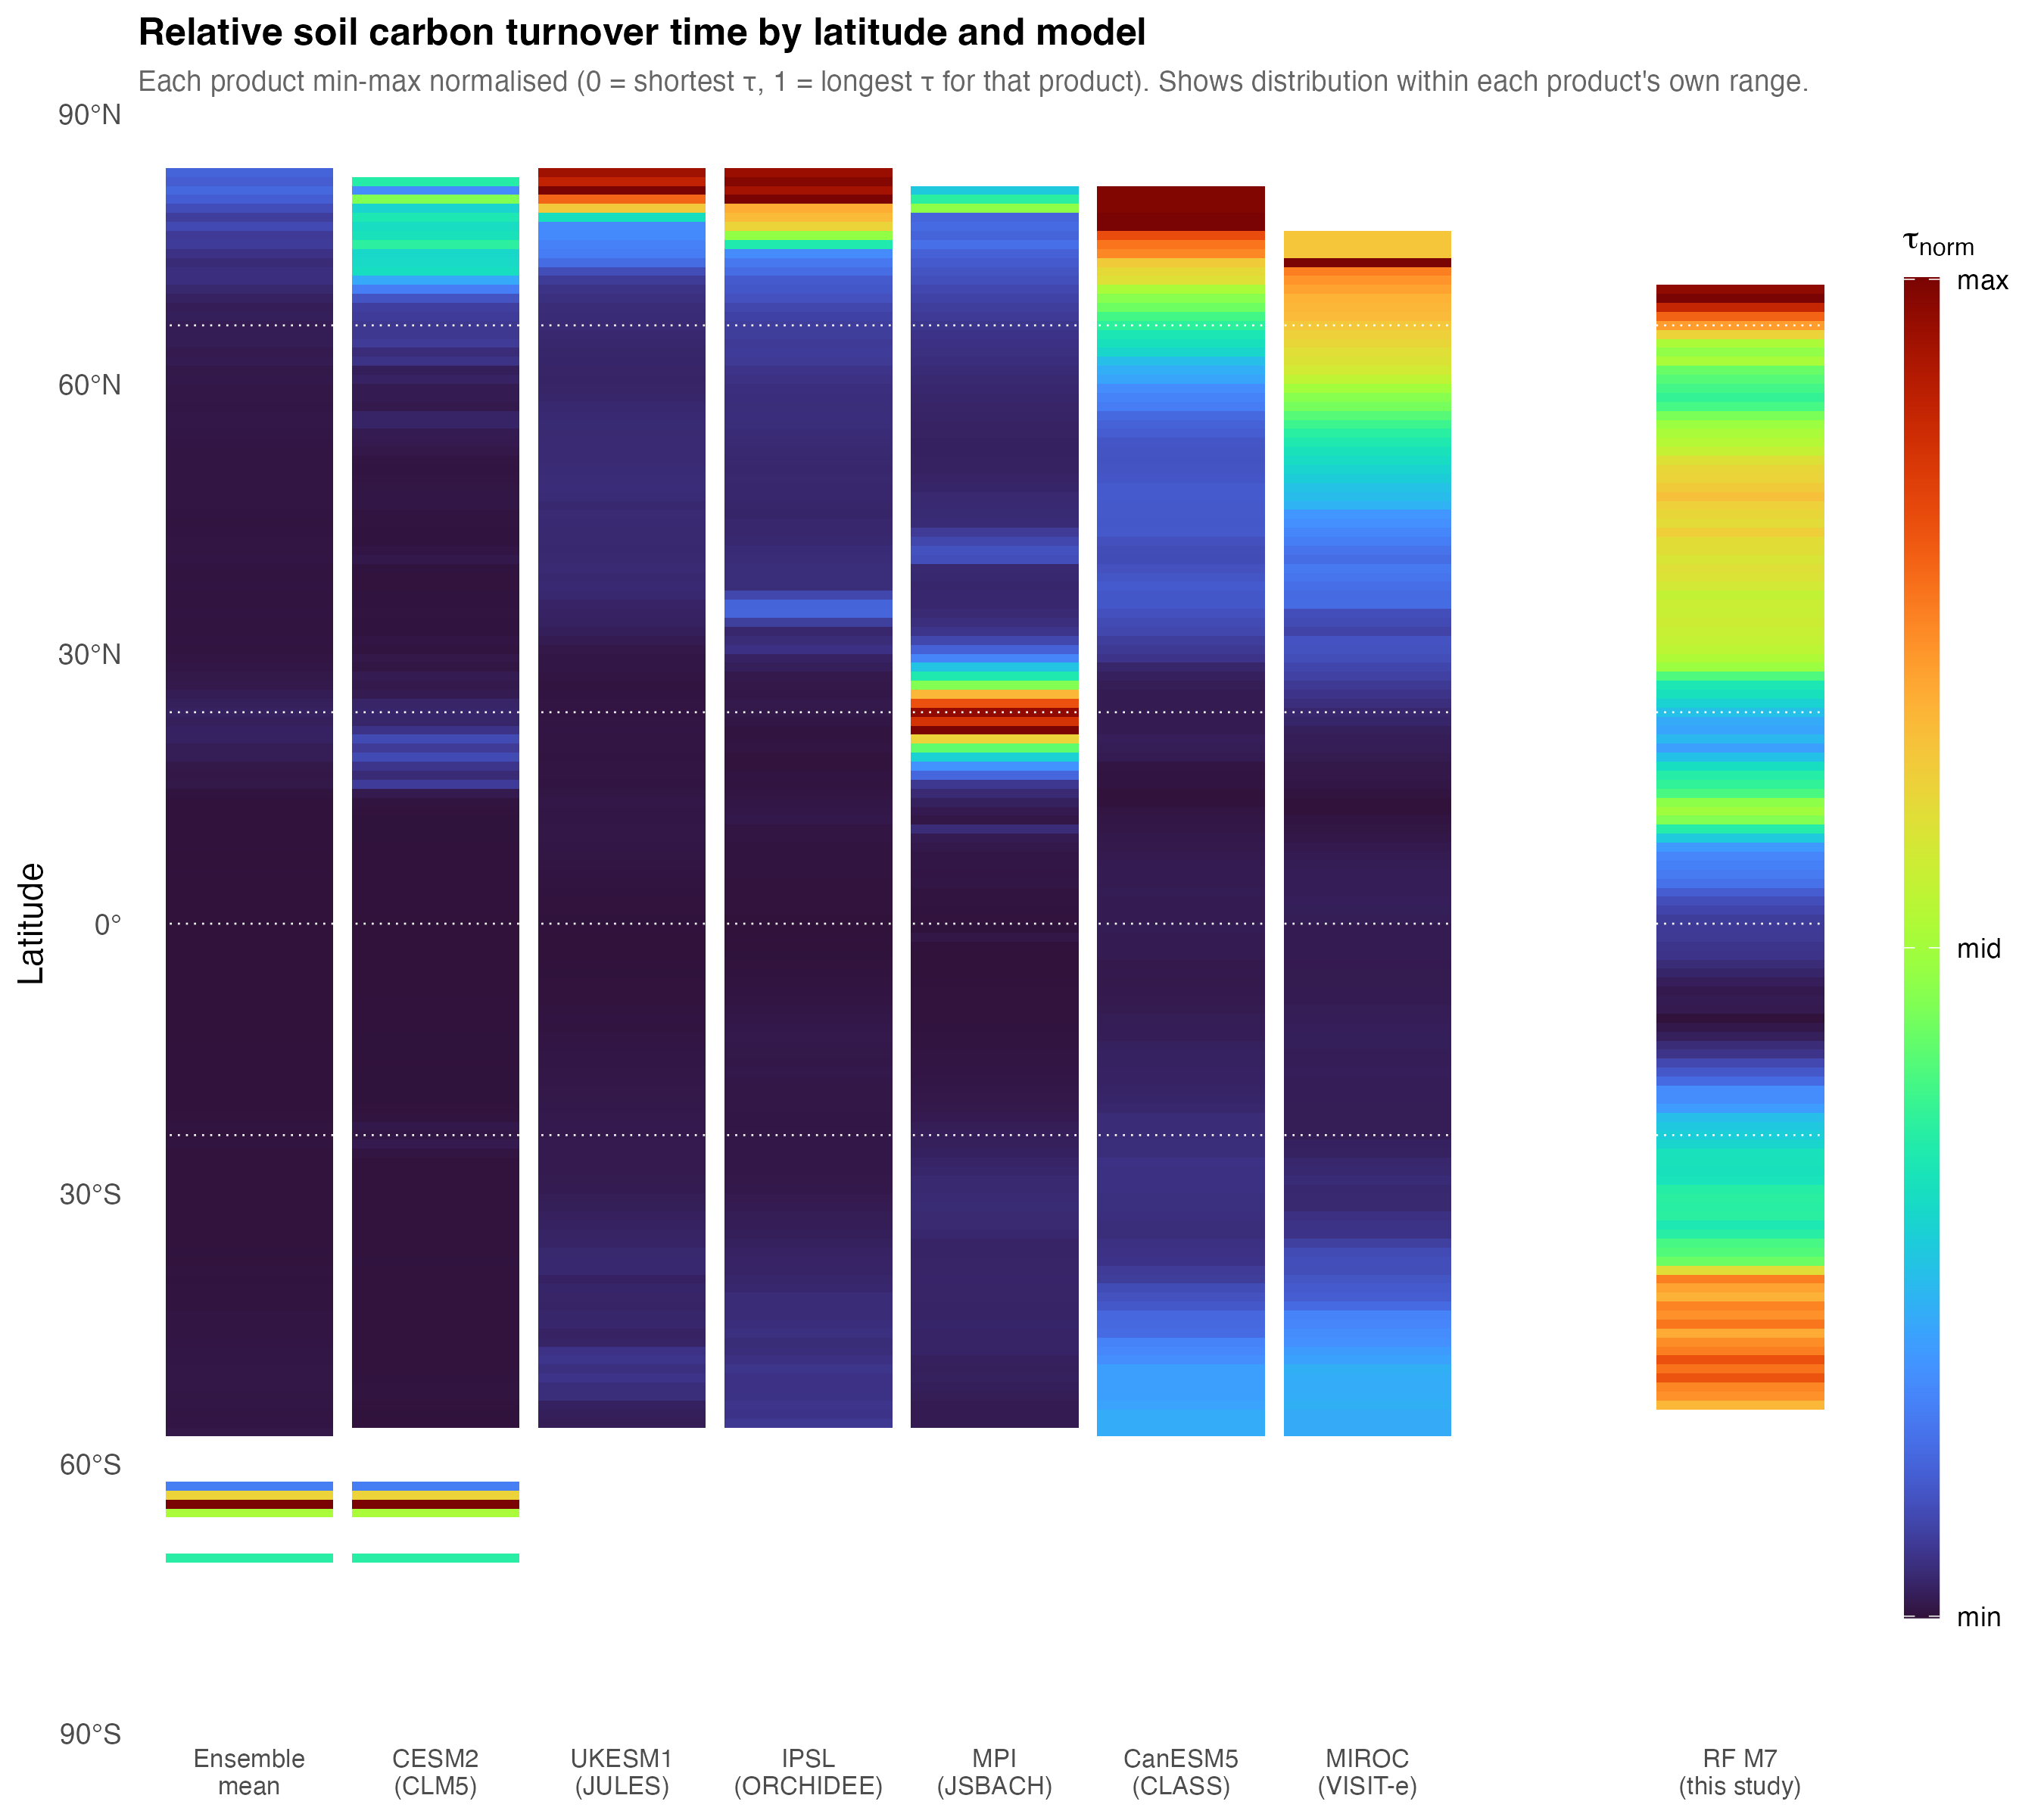
\includegraphics[width=0.92\textwidth]{../plots/step_20/fig_latitude_heatmap_relative.png}
\caption{\textbf{Relative latitudinal structure across the CMIP6 ensemble and this
study.} Each column min--max normalised. The models place most of their structure in
a narrow high-northern band; this study distributes it across latitudes.}
\label{edfig:esm_heatmap}
\end{figure}

\begin{figure}[H]\centering
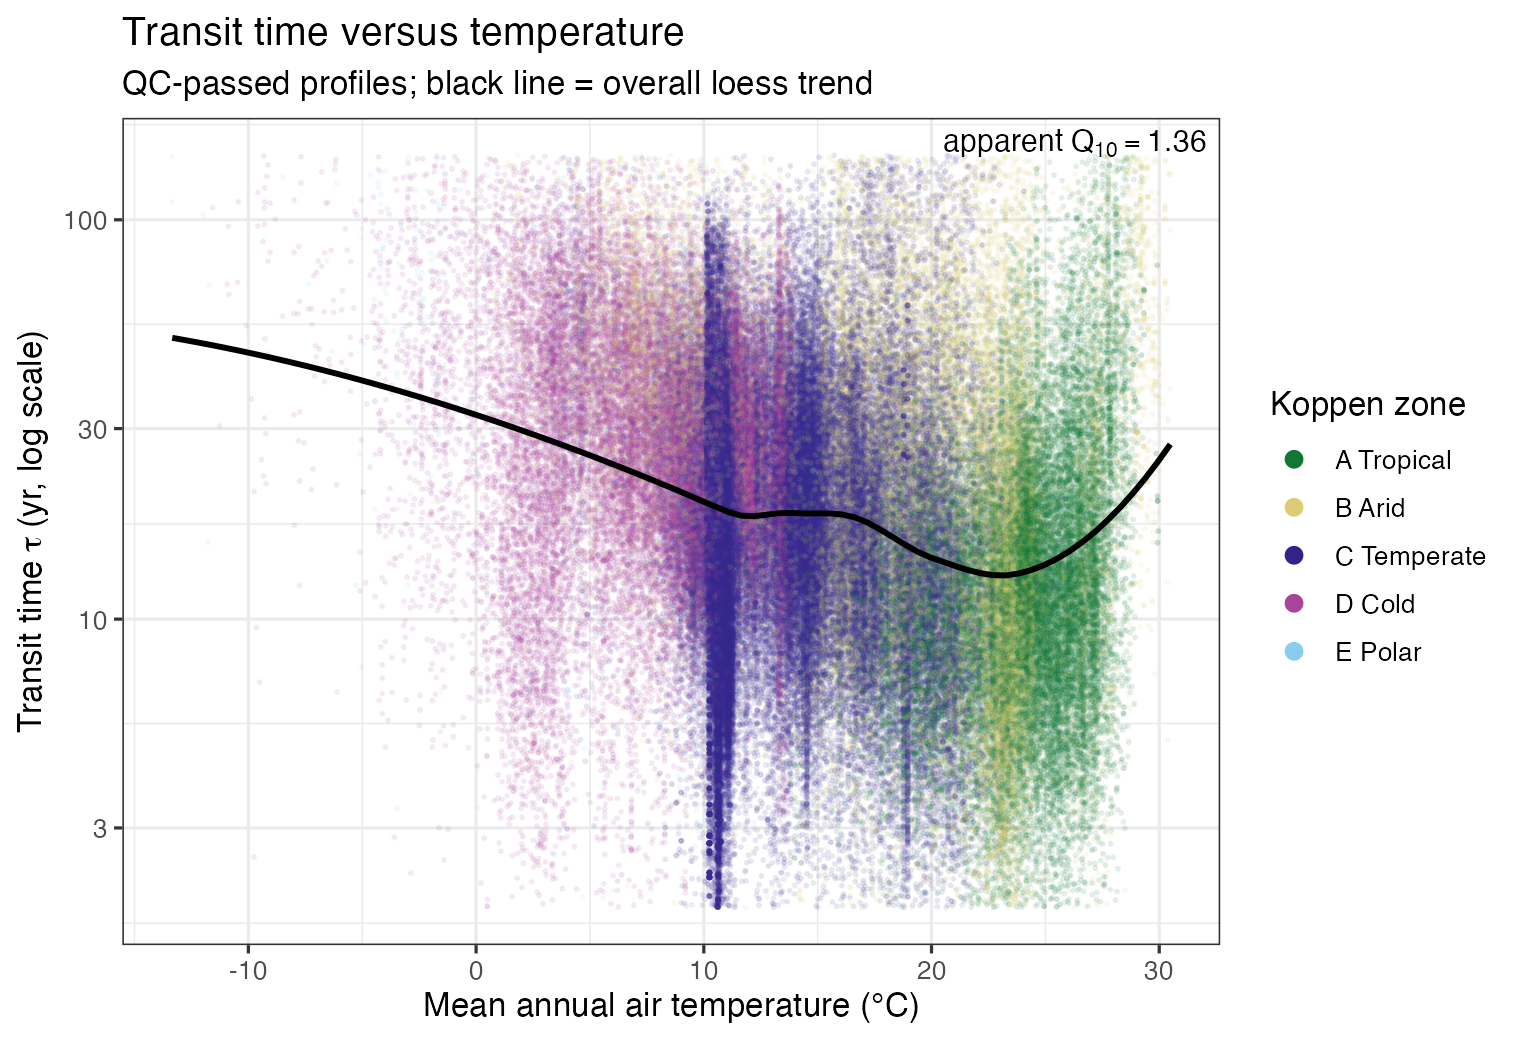
\includegraphics[width=0.75\textwidth]{../plots/appendix/22_temperature_tau_scatter.png}
\caption{\textbf{Transit time versus temperature.} Observed $\tau$ (log scale)
against mean annual air temperature, coloured by coarse K\"oppen zone, with a loess
trend. The weak fit ($R^2=0.06$) shows that temperature alone explains little of the
point-level variation in $\tau$; shown for comparability with earlier compilations
\citep[e.g.][]{Varney2020}.}
\label{edfig:tempscatter}
\end{figure}

\begin{table}[h!]
  \centering\small
  \caption{\textbf{Predictor variables in the full model, by mechanistic group.}
  All variables resampled to $0.1^{\circ}$ for global prediction. Biological rows
  marked $\dagger$ are used only in the nine-layer sensitivity, not in the main
  model.}
  \label{edtab:predictors}
  \begin{tabularx}{\textwidth}{lllX}
    \toprule
    Group & Variable & Units & Source \\
    \midrule
    \multirow{6}{*}{\rotatebox{90}{\textbf{Climate}}}
      & Soil temperature (0--20\,cm)    & \textdegree{}C    & ERA5-Land (depth-weighted stl1/stl2) \\
      & Temperature seasonality         & K     & ERA5-Land (monthly SD of t2m) \\
      & Soil moisture (0--20\,cm)       & m$^3$\,m$^{-3}$ & ERA5-Land (depth-weighted swvl1/swvl2) \\
      & Snow cover fraction             & 0--1             & ERA5-Land \\
      & Potential evaporation            & m                & ERA5-Land \\
      & K\"oppen-Geiger zone            & 1--30            & \citet{Beck2023}, 1991--2020 \\
    \midrule
    \multirow{13}{*}{\rotatebox{90}{\textbf{Edaphic}}}
      & Clay content                    & \%               & SoilGrids 250\,m v2.0, 0--20\,cm \\
      & Sand content                    & \%               & SoilGrids 250\,m v2.0, 0--20\,cm \\
      & Bulk density                    & kg\,dm$^{-3}$    & SoilGrids 250\,m v2.0, 0--20\,cm \\
      & Coarse fragment volume          & \%               & SoilGrids 250\,m v2.0, 0--20\,cm \\
      & pH (H$_2$O)                     & ---              & SoilGrids 250\,m v2.0, 0--20\,cm \\
      & Cation exchange capacity        & cmol\,kg$^{-1}$  & SoilGrids 250\,m v2.0, 0--20\,cm \\
      & Total nitrogen                  & g\,kg$^{-1}$     & SoilGrids 250\,m v2.0, 0--20\,cm \\
      & WRB functional group            & 1--8             & SoilGrids WRB, reclassified \\
      & Elevation                       & m                & Copernicus GLO-30 DEM \\
      & Slope                           & \textdegree{}     & Copernicus GLO-30 DEM \\
      & Northness                       & $-1$ to $+1$     & Copernicus GLO-30 DEM \\
      & Eastness                        & $-1$ to $+1$     & Copernicus GLO-30 DEM \\
      & Terrain ruggedness              & m                & Copernicus GLO-30 DEM (focal SD) \\
    \midrule
    \multirow{8}{*}{\rotatebox{90}{\textbf{Land Use}}}
      & Tree cover fraction             & 0--1             & ESA WorldCover 2021 \\
      & Grassland fraction              & 0--1             & ESA WorldCover 2021 \\
      & Shrubland fraction              & 0--1             & ESA WorldCover 2021 \\
      & Cropland fraction               & 0--1             & ESA WorldCover 2021 \\
      & Bare/sparse fraction            & 0--1             & ESA WorldCover 2021 \\
      & Wetland fraction                & 0--1             & ESA WorldCover 2021 \\
      & Forest loss (binary)            & 0/1              & Hansen GFC v1.10 \\
      & Fire count (pre-sampling)       & count            & MODIS MCD64A1, 2001--2020 \\
    \midrule
    \multirow{9}{*}{\rotatebox{90}{\textbf{Biological}}}
      & Fungal proportion               & 0--1             & \citet{Yu2022} \\
      & AM root colonisation$^\dagger$  & \%               & \citet{Barcelo2023} \\
      & EcM root colonisation$^\dagger$ & \%               & \citet{Barcelo2023} \\
      & EcM:AM root ratio$^\dagger$     & ---              & Derived from above \\
      & AM fungal richness              & index            & \citet{VanNuland2025} (SPUN) \\
      & EcM fungal richness             & index            & \citet{VanNuland2025} (SPUN) \\
      & AM endemism (RWR)               & index            & \citet{VanNuland2025} (SPUN) \\
      & EcM endemism (RWR)              & index            & \citet{VanNuland2025} (SPUN) \\
      & EcM:AM richness ratio           & ---              & Derived from above \\
    \bottomrule
  \end{tabularx}
\end{table}

\begin{table}[h!]
\centering\small
\caption{\textbf{Carbon-input sensitivity of the beyond-climate signal.} The input
coefficient is re-derived on the same NPP field under three conventions (belowground,
total NPP, and total minus a generous forest-harvest export $h$). Block-CV $R^2$, the
beyond-climate gap, Moran's $I$, and the four Shapley shares are all but unchanged;
only the land-use share responds, as expected for a land-cover-structured
coefficient.}
\label{edtab:input}
\begin{tabular}{lrccccrrrr}
\toprule
 & & \multicolumn{2}{c}{Block-CV $R^2$} & Gap & Moran's & \multicolumn{4}{c}{Shapley share (\%)} \\
\cmidrule(lr){3-4}\cmidrule(lr){7-10}
Convention & $n$ & full & clim. & (pp) & $I$ & C & E & B & L \\
\midrule
Belowground (main) & 150,863 & 0.390 & 0.319 & 7.1 & 0.253 & 35.4 & 32.7 & 22.2 & 9.6 \\
Total NPP & 148,714 & 0.389 & 0.319 & 6.9 & 0.260 & 36.3 & 31.6 & 21.5 & 10.6 \\
Total $-$ harvest ($h{=}0.5$) & 149,207 & 0.390 & 0.302 & 8.8 & 0.256 & 34.0 & 32.9 & 21.6 & 11.4 \\
\bottomrule
\end{tabular}
\end{table}

\end{document}
